\documentclass[a4paper,11pt]{article}
\linespread{1.0}
\pdfoutput=1
%\usepackage[latin1]{inputenc}
\usepackage[utf8]{inputenc}
\usepackage{amssymb}
\usepackage{amsmath}
\usepackage{amsthm}
\usepackage{amsfonts}
\usepackage[pdftex]{graphicx}
\usepackage{geometry}
\usepackage{braket}
\usepackage{enumerate}
\usepackage{comment}


%*** RESIDUE ***
\DeclareMathOperator*{\Res}{Res}
\DeclareMathOperator{\Li}{Li_2}
%***************
\usepackage{subcaption}

\allowdisplaybreaks

%\usepackage[usenames,dvipsnames]{xcolor}
\usepackage[table,usenames,dvipsnames]{xcolor}

%\pagestyle{plain}
\usepackage{setspace}
\usepackage[in]{fullpage}
\usepackage{hyperref}
\usepackage{array}
\usepackage{cancel}
\usepackage{wrapfig}
\usepackage[font=small,labelfont=bf]{caption}
\usepackage{pifont}
\newcommand{\cmark}{\ding{51}}
\newcommand{\xmark}{\ding{55}}
\usepackage[dvipsnames]{xcolor}
\usepackage{mathtools}
% \usepackage{todonotes}

\usepackage{color}

\usepackage{tikz}
\usetikzlibrary{arrows,shapes}
\usetikzlibrary{trees}
\usetikzlibrary{matrix,arrows} % For commutative diagram
\usetikzlibrary{positioning}% For "above of=" commands
\usetikzlibrary{calc,through}% For coordinates
\usetikzlibrary{decorations.pathreplacing}% For curly braces
\usepackage{pgffor}	% For repeating patterns

\numberwithin{equation}{section}

\usepackage[english]{babel}

\usepackage{slashed}
\usepackage{caption}

\usepackage[nottoc,notlot,notlof]{tocbibind}
\usepackage[nosort]{cite}   
\usepackage{color}


\usepackage{parskip}
\setlength{\parindent}{10pt}
\setlength{\parskip}{1.9mm}

\usepackage[T1]{fontenc}

\usepackage{lmodern}
\usepackage{sectsty}
\usepackage{yfonts}
\allsectionsfont{\boldmath}

\usepackage{physics}
\usepackage{slashed}
\usepackage{makeidx}
\usepackage[vcentermath]{youngtab}
\usepackage{amsthm}
\usepackage[scr=boondoxo]{mathalfa}

\hypersetup{
	colorlinks=true,
	linktoc=page,
	citecolor=blue,
	linkcolor=blue,
	urlcolor=blue} 

\urlstyle{same}

\usepackage{tikz}
\usetikzlibrary{arrows,shapes}
\usetikzlibrary{trees}
\usetikzlibrary{matrix,arrows} 				% For commutative diagram
											% http://www.felixl.de/commu.pdf
\usetikzlibrary{positioning}				% For "above of=" commands
\usetikzlibrary{calc,through}				% For coordinates
\usetikzlibrary{decorations.pathreplacing}  % For curly braces
% http://www.math.ucla.edu/~getreuer/tikz.html
\usepackage{pgffor}							% For repeating patterns

\usetikzlibrary{decorations.pathmorphing}	% For Feynman Diagrams
\usetikzlibrary{decorations.markings}
\tikzset{
	% >=stealth', %%  Uncomment for more conventional arrows
   % vector/.style={decorate, decoration={snake}, draw},
   vector/.style={decorate, decoration={snake, amplitude=1pt, segment length=6pt}, draw,double},
	provector/.style={decorate, decoration={snake,amplitude=2.5pt}, draw},
	antivector/.style={decorate, decoration={snake,amplitude=-2.5pt}, draw},
    fermion/.style={draw=black, postaction={decorate},
        decoration={markings,mark=at position .55 with {\arrow[draw=black]{>}}}},
    fermionbar/.style={draw=black, postaction={decorate},
        decoration={markings,mark=at position .55 with {\arrow[draw=black]{<}}}},
    fermionnoarrow/.style={draw=black},
    gluon/.style={decorate, draw=black,
        decoration={coil,amplitude=4pt, segment length=5pt}},
    scalar/.style={dashed,draw=black, postaction={decorate},
        decoration={markings,mark=at position .55 with {\arrow[draw=black]{>}}}},
    scalarbar/.style={dashed,draw=black, postaction={decorate},
        decoration={markings,mark=at position .55 with {\arrow[draw=black]{<}}}},
    scalarnoarrow/.style={dashed,draw=black},
    electron/.style={draw=black, postaction={decorate},
        decoration={markings,mark=at position .55 with {\arrow[draw=black]{>}}}},
	bigvector/.style={decorate, decoration={snake,amplitude=4pt}, draw},
}
%Manuel added this for crosses
\tikzset{cross/.style={cross out, draw, 
         minimum size=2*(#1-\pgflinewidth), 
         inner sep=0pt, outer sep=0pt}}

% TIKZ - for block diagrams, 
% from http://www.texample.net/tikz/examples/control-system-principles/
% \usetikzlibrary{shapes,arrows}
\tikzstyle{block} = [draw, rectangle, 
    minimum height=3em, minimum width=6em]

%%%%%%%%

%%%% Nice bullet %%%%

\newcommand*{\sagex}{
     \item[{\includegraphics[scale=0.05]{Sagex.png}}]
    }

%%%% Some definition for the spinor braket in four and six dimensions %%%%%

\newcommand{\agl}[2]{\langle#1 #2 \rangle}
\newcommand{\sqr}[2]{\lbrack #1 #2 \rbrack}
\newcommand{\sabr}[4]{[#1_{\dot{#2}} #3_{#4}\rangle}
\newcommand{\asbr}[4]{\langle#1_{#2} #3_{\dot{#4}}]}
\newcommand{\afour}[8]{\langle#1_{#2} #3_{#4} #5_{#6} #7_{#8} \rangle}
\newcommand{\bfour}[8]{[#1_{\dot{#2}} #3_{\dot{#4}} #5_{\dot{#6}} #7_{\dot{#8}}]}

\newcommand{\lu}[1]{\lambda^{#1}}
\newcommand{\ltu}[1]{\tilde{\lambda}^{\dot{#1}}}
\newcommand{\ld}[1]{\lambda_{#1}}
\newcommand{\ltd}[1]{\tilde{\lambda}_{\dot{#1}}}
\newcommand{\muu}[1]{\mu^{#1}}
\newcommand{\mtu}[1]{\tilde{\mu}^{\dot{#1}}}
\newcommand{\mud}[1]{\mu_{#1}}
\newcommand{\mtd}[1]{\tilde{\mu}_{\dot{#1}}}

%%%% Some useful character %%%%

\newcommand{\RR}{\mathbb{R}}
\newcommand{\CC}{\mathbb{C}}
\newcommand{\cA}{\mathcal{A}}
\newcommand{\cN}{\mathcal{N}}
\newcommand{\cL}{\mathcal{L}}
\newcommand{\cO}{\mathcal{O}}
\newcommand{\tb}{\tilde{b}}

%%%% Manuel's packages %%%%

\usepackage{float}
\usepackage{marvosym}
\usepackage{empheq}
\usepackage{bbold}

%%%% Manuel's fancyref and tikz %%%%

\usepackage{tikz}
\usetikzlibrary{shapes}
\usetikzlibrary{arrows}
\usetikzlibrary{positioning}
\usetikzlibrary{decorations.pathmorphing}
\usetikzlibrary{decorations.pathreplacing}
\usetikzlibrary{decorations.markings}

%%%%%%% Gab's extra definitions %%%%%%

%%%%                    DEFINITIONS

%%%%%%%%%%%%%%%%%%%%%%%%%%%%%%%%%%%%%%%%%%%%%%%%%%%%%%%
%%                      Commands

% \newcommand{\be}{\begin{equation}}
% \newcommand{\ee}{\end{equation}}
% \newcommand{\eq}[1]{(\ref{#1})}
% \newcommand{\hf}{\frac{1}{2}}
% \newcommand{\nn}{\nonumber\\}

% \def\beqa{\begin{eqnarray}}
% \def\eeqa{\end{eqnarray}}
% \def\beq{\begin{equation}}
% \def\eeq{\end{equation}}
% \def\sst{\scriptscriptstyle}
% \def\thetabar{\bar\theta}
% \def\Tr{{\rm Tr}}
% \def\one{\mbox{1 \kern-.59em {\rm l}}}
% \def\Nh{\hat{N}}

 \def\cA{\mathcal{A}}
 \def\uno{\mbox{1 \kern-.59em {\rm l}}}

\newcommand{\half}{{\textstyle {\genfrac{1}{2}}}}

%%%%%%%%%%%


\begin{document}

%%%% Title page %%%%

\begin{flushright}
	QMUL-PH-20-05\\
	SAGEX-20-04-E\\
	%HU-EP-18/25
\end{flushright}

\vspace{20pt} 

\begin{center}

		
	%{\Large \bf  Newton potential in $R^2$ gravity revisited   }  \\
	{\Large \bf  Eikonal phase matrix, deflection angle and time delay}  \\
	\vspace{0.3 cm} {\Large \bf  in effective field theories of gravity}


	\vspace{25pt}

	{\mbox {\sf  \!\!\!\!Manuel~Accettulli~Huber, Andreas~Brandhuber, Stefano~De~Angelis and 				Gabriele~Travaglini{\includegraphics[scale=0.05]{Sagex.jpeg}}
	}}
	\vspace{0.5cm}

	\begin{center}
		{\small \em
			Centre for Research in String Theory\\
			School of Physics and Astronomy\\
			Queen Mary University of London\\
			Mile End Road, London E1 4NS, United Kingdom
		}
	\end{center}

	%\vspace{-8pt}

	\vspace{40pt}  %was 40 

	{\bf Abstract}
	%
\end{center}

\vspace{0.3cm}

\noindent

\noindent



We could use this one? $\mathscr{b}$     $\mathscr{q}$      $\mathscr{\bar{q}}$  

Abstract here

 
\vfill
\hrulefill
\newline
\vspace{-1cm}
${\includegraphics[scale=0.05]{Sagex.jpeg}}$~\!\!{\tt\footnotesize\{m.accettullihuber, a.brandhuber, s.deangelis, g.travaglini\}@qmul.ac.uk}

\setcounter{page}{0}
\thispagestyle{empty}
\newpage

%%%%%%%%%%%%%%%%%% TABLE OF CONTENTS %%%%%%%%%%%%%%%%%%%%%%%%%%%%%%%%%

\setcounter{tocdepth}{4}
\hrule height 0.75pt
\tableofcontents
\vspace{0.8cm}
\hrule height 0.75pt
\vspace{1cm}
\setcounter{tocdepth}{2}

\newpage
%%%%%%%%%%%%%%%%%%%%%%%%%%%%%%%%%%%%%%%%%%%%%%%%%%%%%%%%%%%
\section{Introduction} 

We start with the action
\begin{align}
\begin{split}
\label{action}
S = \int\!\dd[4] x\sqrt{-g} \,  \bigg[ &-\frac{2}{\kappa^2}R   \, - \, \frac{1}{4} F^{\mu \nu} F_{\mu\nu}\, +\, \frac{1}{2} (D_{\mu} \phi)( D^{\mu}\phi) - \frac{1}{2} m^2 \phi^2\\
&- \,  {2\over \kappa^2} \left( {\alpha^{\prime \, 2} \over 48} \, I_1 + {\alpha^{\prime \, 2} \over 24} \, G_3 \right) \, - \, \alpha_{\gamma} \, F^{\mu\nu} F^{\rho \sigma} R_{\mu \nu \rho \sigma} \, + \, \alpha_{4}``R^4 " \bigg] \, , 
\end{split}
\end{align}
where $I_1 := {R^{\alpha \beta}}_{\mu \nu} {R^{\mu \nu}}_{\rho \sigma} {R^{\rho \sigma}}_{\alpha \beta}$
and $G_3 := I_1 - 2 {R^{\mu \nu \alpha}}_\beta {R^{\beta \gamma}}_{\nu \sigma} {R^\sigma}_{\mu \gamma \alpha}$, 
while  $``R^4"$ stands for the 
\textcolor{green}{Stefano: Please correct as appropriate. How many different structures are there in 4D and are the all plus and MHV 4-point amplitudes independent or linked!?} 

\textcolor{red}{I have removed Einstein-Hilbert and used   EH instead, apart from within the title of a section. We should remember to call it Einstein-Hilbert the first time!}


\section{From amplitudes  to the deflection angle  and time delay via the eikonal}

In this paper we are mainly interested in the elastic bending of a graviton in the background produced by
a heavy scalar particle. The means to this
goal will be the study of scattering amplitudes in the eikonal  approximation, which corresponds to a highly forward high-energy scattering such that the center of mass energy is much larger than the momentum transfer. In this section we first give a more precise definition of this kinematic limit providing explicit parametrisations for all the quantities we will need later on. Then we briefly review the connection between the amplitude in such limit, also known as the eikonal approximation, and the so called eikonal phase, which can be shown to be directly related to the bending angle in an appropriate two-dimensional space called impact parameter space.



\subsection{Kinematics of the scattering}

In this  section we describe the kinematics of the scattering processes we  consider. We denote by  $p_1$ and $p_2$  the four-momenta of the incoming and outgoing scalars, respectively, with  $m$ being their common mass. The momenta of the incoming and outgoing  gravitons are denoted by $p_4$ and $p_3$, respectively. We will  work in the centre of mass frame, with the following parameterisation: 
%\begin{figure}[h]
%\centering
%\begin{tikzpicture}[scale=15]
%\def\x{0}
%\def\y{0}
%
%\node at (0+\x,0+\y) (centro) {};
%\node at (-3pt+\x,-3pt+\y) (uno) {$p_1$};
%\node at (-3pt+\x,3pt+\y) (due) {$p_2$};
%\node at (3pt+\x,3pt+\y) (tre) {$p_3^{h_3}$};
%\node at (3pt+\x,-3pt+\y) (quat) {$p_4^{h_4}$};
%
%\draw [thick] (uno) -- (centro);
%\draw [thick] (due) -- (centro);
%\draw [vector,double] (tre) -- (centro);
%\draw [vector,double] (quat) -- (centro);
%
%\draw [->] (-2.8pt+\x,-2pt+\y) -- (-1.8pt+\x,-1pt+\y); 
%\draw [->] (2.8pt+\x,-2pt+\y) -- (1.8pt+\x,-1pt+\y); 
%\draw [->] (-1.8pt+\x,1pt+\y) -- (-2.8pt+\x,2pt+\y); 
%\draw [->] (1.8pt+\x,1pt+\y) -- (2.8pt+\x,2pt+\y); 
%
%%\node at (0+\x,0+\y) [draw, fill=gray!90!black, circle, inner sep=10pt] {};
%
%\shade [shading=radial] (centro) circle (1.5pt);
%
%\end{tikzpicture}
%\end{figure}


%In this frame  
%\begin{align}
%\begin{split}
%\label{kinematics}
%p_4^\mu & = - (E_4,-\vec{p}+\vec{q}/2)\, ,  \\
% p_1^\mu & =  -(E_1,\vec{p}-\vec{q}/2) \, , \\
%p_2^\mu & =  (E_2,\vec{p}+\vec{q}/2) \, ,  \\
%p_3^\mu & =  (E_3,-\vec{p}-\vec{q}/2)\ .
%\end{split}
%\end{align}

\begin{equation}\label{kinematics}
\begin{array}{lr}

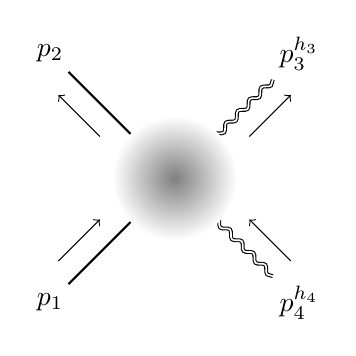
\begin{tikzpicture}[scale=15,baseline={([yshift=-1mm]centro.base)}]
\def\x{0}
\def\y{0}

\node at (0+\x,0+\y) (centro) {};
\node at (-3pt+\x,-3pt+\y) (uno) {$p_1$};
\node at (-3pt+\x,3pt+\y) (due) {$p_2$};
\node at (3pt+\x,3pt+\y) (tre) {$p_3^{h_3}$};
\node at (3pt+\x,-3pt+\y) (quat) {$p_4^{h_4}$};

\draw [thick] (uno) -- (centro);
\draw [thick] (due) -- (centro);
\draw [vector,double] (tre) -- (centro);
\draw [vector,double] (quat) -- (centro);

\draw [->] (-2.8pt+\x,-2pt+\y) -- (-1.8pt+\x,-1pt+\y); 
\draw [->] (2.8pt+\x,-2pt+\y) -- (1.8pt+\x,-1pt+\y); 
\draw [->] (-1.8pt+\x,1pt+\y) -- (-2.8pt+\x,2pt+\y); 
\draw [->] (1.8pt+\x,1pt+\y) -- (2.8pt+\x,2pt+\y); 

%\node at (0+\x,0+\y) [draw, fill=gray!90!black, circle, inner sep=10pt] {};

\shade [shading=radial] (centro) circle (1.5pt);

\end{tikzpicture}
&\hspace{2cm}
\begin{aligned}
p_4^\mu & = - (E_4,-\vec{p}+\vec{q}/2)\, ,  \\
 p_1^\mu & =  -(E_1,\vec{p}-\vec{q}/2) \, , \\
p_2^\mu & =  (E_2,\vec{p}+\vec{q}/2) \, ,  \\
p_3^\mu & =  (E_3,-\vec{p}-\vec{q}/2)\ .
\end{aligned}

\end{array}
\end{equation}
In our conventions we take all momenta to be outgoing, hence the minus signs in the expressions of  $p_1$ and $p_4$ since particles 1 and 4 are incoming. 
We also have 
\begin{align}
\begin{split}
\label{enbend}
E_1&=E_2 =\sqrt{m^2+\vec{p}^{\, \, 2}+\vec{q}^{\, \, 2}/4}\, , 
\\
E_3&=E_4=\sqrt{\vec{p}^{\,\,   2}+\vec{q}^{\, \, 2}/4}\,  := \, \omega
\ ,
\end{split}
\end{align}
 where  $\vec{p} \, \cdot \, \vec{q}=0$ due to momentum conservation.  Hence $\vec{q}$\,
lives in a two-dimensional space orthogonal to $\vec{p}$.
%
 In this paper  we  define  the  Mandelstam variables as
 \begin{align}
\label{mandel}
s:=(p_1+p_2)^2 = -\vec{q}^{\, \, 2}   , \ \  \ t:=(p_1+p_4)^2 = (E_1+E_4)^2  ,  
 \ \ \ u:=(p_1+p_3)^2  , 
 \end{align}
with $s+t+u = 2 m$.
In this notation, the spacelike momentum transfer squared is given by $s$, while $t$ denotes the centre of mass
energy squared, and $\omega$ is the energy of the scattered massless particle.


In the above  parameterisation, the kinematic limit we are interested  is  
\begin{align}
\begin{split}
\label{bendlim}
m\gg \omega \gg |\vec{q}\, |
\ ,
\end{split}
\end{align}
which implies for the Mandelstam variables
\begin{equation}
t \simeq m^2 + 2m \omega \>, \hspace{1cm} ut - m^4 \simeq - (2 m \omega)^2 \>,
\end{equation}
and for the graviton energies
\begin{align}
\begin{split}
E_3=E_4 := \omega \simeq |\vec{p}\, |\left(1 + {\vec{q}^{\, \, 2} \over 8 \,\vec{p}^{\, \, 2}}\right)
\ .
\end{split}
\end{align}
We will consider the gravitons to be strongly boosted along a certain direction, say the $\hat{z}$ axis, which we can achieve by taking 
$\vec{p} = |\vec{p}\,|\, \hat{z}$ with $|\vec{p}\, |\gg |\vec{q}\, |$.
In the  kinematic limit \eqref{bendlim} we can write the four-momentum $p_3$ of the scattered graviton in spinor notation as 
\begin{align}
\label{spainors}
\begin{split}
p_3 = \begin{pmatrix} 
\dfrac{\vec{q}^{\, \, 2}}{  8  |\vec{p}\, |}  & - \dfrac{\bar{q}}{2}
\vspace{0.3cm} \\ 
- \dfrac{{q}}{2}  & 2  |\vec{p}\, |
\end{pmatrix} \, , 
\end{split}
\end{align}
with $q:= q_1 + i q_2$ and $\bar{q}:= q_1 - i q_2$.  One can then find an explicit parameterisation for the spinors associated to the two graviton momenta  $p_i=\lambda_i \tilde{\lambda}_i$, $i=3,4$, with 
the result 
\begin{align}
\begin{split}
\lambda_3 &= \sqrt{ 2  |\vec{p}\, |} 
\begin{pmatrix} 
 - \dfrac{\bar{q}}{ 4   |\vec{p}\, |}
\vspace{0.3cm} \\ 
1
\end{pmatrix} \ , \qquad 
\ \, \tilde{\lambda}_3 = \sqrt{ 2  |\vec{p}\, |} 
\begin{pmatrix} 
 - \dfrac{{q}}{ 4   |\vec{p}\, |} & 
\hspace{0.3cm}  
1
\end{pmatrix} \ , 
\\
\lambda_4 &=i \sqrt{ 2  |\vec{p}\, |} 
\begin{pmatrix} 
  \dfrac{\bar{q}}{ 4   |\vec{p}\, |}
\vspace{0.3cm} \\ 
1
\end{pmatrix} \ , \qquad \quad
\tilde{\lambda}_4 = i\sqrt{ 2  |\vec{p}\, |} 
\begin{pmatrix} 
  \dfrac{{q}}{ 4   |\vec{p}\, |} & 
\hspace{0.3cm}  
1
\end{pmatrix} \ .
\end{split}
\end{align}
Note the extra factors of $i$ due to the negative zero-component of $p_4$ corresponding to an incoming particle.

\subsection{Eikonal phase, deflection angle and time delay}

In this section we briefly review some concepts related to the eikonal approximation and the computation  of the deflection angle from scattering amplitudes in this approximation. This topic has received renewed attention in the late sixties and a vast  literature exists, for which we refer the interested reader to~\cite{DiVecchia:2019myk,DiVecchia:2019kta,KoemansCollado:2019ggb} and references therein.

The scattering amplitude in impact parameter space $\widetilde{\cA}$ is defined as a  Fourier transform of the amplitude $\mathcal{A}$ with respect to the  momentum transfer  $\vec{q}$, 
\begin{align}
\label{amptraimp}
\widetilde{\cA} (\vec{b}\,) \ := \ {1\over 4 m \,\omega} \int\!{d^{D-2} q\over (2 \pi)^{D-2}} \, e^{i \vec{q} \cdot \vec{b}} \ \cA (\vec{q}\,)\ , 
\end{align}
where $\vec{b}$ is the impact parameter, and the number of dimensions will eventually be set  to $D=4-2\epsilon$.

In the eikonal approximation it is expected that the $S$-matrix can be written in the form \cite{Amati:1990xe}
\begin{align}
\label{eq:Seikonal0}
S_{\rm eik} = 
e^{i (\delta_0+ \delta_1+ \ldots ) }
\ , 
\end{align} 
where $\delta_0$ is the leading eikonal phase, which is of $\mathcal{O}(G)$, $\delta_1$ the first subleading correction, which is of $\mathcal{O}(G^2)$,  and the dots represent  subsubleading contributions. On the other hand, one can also write the $S$-matrix in impact parameter space as
\begin{align}
\label{eq:Seikonal}
S_{\rm eik} \ = \ 1 +  \widetilde{\cA}^{(0)}_{\omega} +  \widetilde{\cA}^{(1)}_{\omega^2} + \widetilde{\cA}^{(1)}_{\omega} + \ldots \ , 
\end{align}
 where the superscript indicates the loop order and the subscript the power in the energy $\omega$ of the emitted graviton. 
Equating \eqref{eq:Seikonal0} with \eqref{eq:Seikonal} one gets
\begin{align} 
\label{delta0}
\delta_0 &= \  -i \, \widetilde{\cA}^{(0)}_{\omega}\ ,\\[.2em]
\label{delta1}
\delta_1 &= \  -i\,  \widetilde{\cA}^{(1)}_{\omega}\ , 
\end{align}
as well as the condition 
\begin{align} 
- {(\delta_0)^2\over 2} \ = \  \widetilde{\cA}^{(1)}_{\omega^2}
\ , 
\end{align}
which implies the consistency condition 
\begin{align}
\label{exponentiation}
\widetilde{\cA}^{(1)}_{\omega^2} \ = \   {1\over 2} (\widetilde{\cA}^{(0)}_{\omega})^2
 \ . 
 \end{align}
Thus, the  leading in $\omega$ contribution to the one-loop amplitude, $\widetilde{\cA}^{(1)}_{\omega^2}$,  does  not provide any new information about the $S$-matrix.  Instead we have to expand the impact parameter amplitude in $\omega$ and extract from it, the quantities   $\delta_0$, $\delta_1$ and so on. We also note that \eqref{delta0}--\eqref{exponentiation} hold as  matrix equations. 



Finally, the particle deflection angle can  be obtained from the eigenvalues $\delta^{(i)}$ of the matrix $\delta$. 
Using a saddle-point approximation \cite{Amati:1990xe, Bjerrum-Bohr:2016hpa,Bjerrum-Bohr:2017dxw} one finds, for small $\theta$, 
\begin{equation}
\label{rebend}
\theta^{(i)}  \ = \ \frac{1}{\omega} \frac{\partial}{\partial b} {\delta^{(i)}} \, , 
\end{equation}
where  $i$ runs over all  eigenvalues of $\delta$ and $b=\abs*{\vec{b}}$. 

\textcolor{red}{ Give formula for time delay as well!! Below is morally correct but needs some factors!?
\begin{equation}
t^{(i)} = \frac{\partial \delta^{(i)}}{\partial \omega}
\ .
\end{equation}
We will also need to add this to each section for the various couplings. A relevant formula seems to be (33) of
\cite{Ciafaloni:2014esa} with $E_p$ being our $\omega$ (please check!). It seems to be consistent with the conclusions drawn below (3.22) of  \cite{Camanho:2014apa}. 
}

%\textcolour{black}}


\section{The relevant scattering amplitudes}

In this section we provide the relevant one-loop amplitudes needed in order to extract the  bending angle. We work in the eikonal approximation \eqref{bendlim}, and the expressions for all amplitudes will be given in that approximation.  
Furthermore, as already mentioned in the previous section, we need only  compute the part of the amplitude with  a discontinuity in the $s$-channel.%
\footnote{We recall that  $s=-|\vec{q}\, |^2$ where  $\vec{q}$ is the  momentum exchange between the classical source and the graviton. }
A direct extraction of the classical part of the bending  angle can also be  performed  using a triple cut, and in an even more refined way using the holomorphic classical limit \cite{Guevara:2017csg}.


\textcolor{green}{Stefano, please produce a figure with the massive triple cut and put below two-particle cut figure. In this section we only state that we have crosschecked all massive triangles from the two-particle cuts also with the triple cut. Give details of one sample computation in the appendix and compare with HCL if relevant/possible! All other details including bubbles to remain, in this section we only give details of the amplitudes so we should keep the complete results (in the eikonal approximation).}\\
For a generic $R^n$ contribution, the two-particle cut diagrams to consider are shown in Figure~\ref{fig:doublecut}.
\begin{figure}[ht]
\centering
    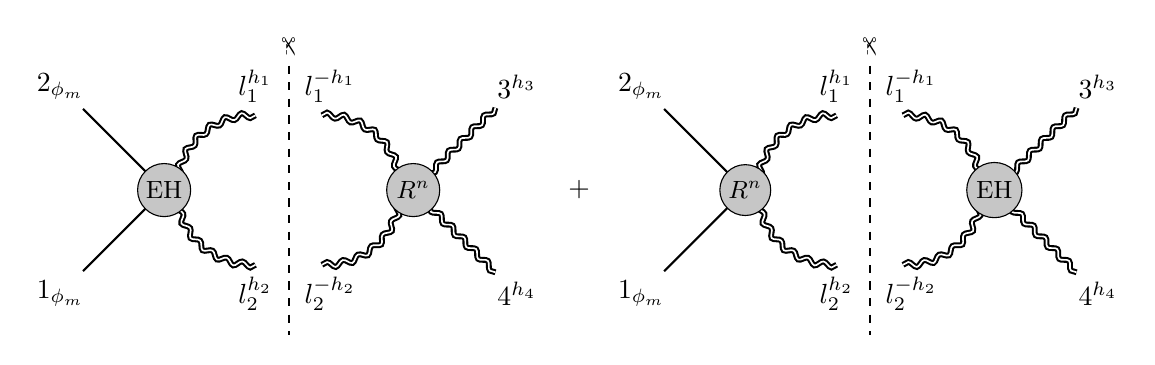
\begin{tikzpicture}[scale=15]

        \def\x{0};
        \def\y{0};
        \node at (0+\x,0+\y) (left) {};
        \node at (-2.5pt+\x,2.5pt+\y) (oneA) {$2_{\phi_m}$};
        \node at (-2.5pt+\x,-2.5pt+\y) (oneB) {$1_{\phi_m}$};
        \node at (1.7pt+\x,1.5pt+\y) (top){};
        \node at (1.7pt+\x,-1.5pt+\y) (bottom){};

        \draw [line width=.75,vector] (2.2pt,1.8pt) arc (90:180:1.8pt);
        \draw [line width=.75,vector] (2.2pt,-1.8pt) arc (270:180:1.8pt);
        \draw [line width=.75] (oneA) -- (left);
        \draw [line width=.75] (oneB) -- (left);
        \node at (0+\x,0+\y) [draw, fill=gray!45!white, circle, inner sep=1.7pt]{\small EH};

        \draw [dashed, line width=.75] (3pt+\x,3pt+\y) -- (3pt+\x,-3.5pt);
        \node at (3.1pt+\x,3.2pt+\y)[rotate around={-90:(1pt,2.5pt)}]{\Cutright};
%        \node at (-2.3pt+\x,0pt+\y) {$m$};

		\node at (2.2pt+\x,2.5pt+\y) {$l_1^{h_1}$};
        \node at (2.2pt+\x,-2.5pt+\y) {$l_2^{h_2}$};



        \def\x{6pt};
        \def\y{0};

        \node at (0+\x,0+\y) (left) {};
        \node at (2.5pt+\x,2.5pt+\y) (oneA) {$3^{h_3}$};
        \node at (2.5pt+\x,-2.5pt+\y) (oneB) {$4^{h_4}$};
        \node at (-1.7pt+\x,1.5pt+\y) (top){};
        \node at (-1.7pt+\x,-1.5pt+\y) (bottom){};

        \draw [line width=.75,vector] (-2.2pt+\x,1.8pt) arc (90:0:1.8pt);
        \draw [line width=.75,vector] (-2.2pt+\x,-1.8pt) arc (270:360:1.8pt);
        \draw [vector,line width=.75] (oneA) -- (left);
        \draw [vector,line width=.75] (oneB) -- (left);
        \node at (0+\x,0+\y) [draw, fill=gray!45!white, circle, inner sep=2pt]{\small $R^n$};
        
        \node at (-2pt+\x,2.5pt+\y) {$l_1^{-h_1}$};
        \node at (-2pt+\x,-2.5pt+\y) {$l_2^{-h_2}$};
       
       \node at (4pt+\x,0+\y) {+};
       
       	\def\x{14pt};
        \def\y{0};
        \node at (0+\x,0+\y) (left) {};
        \node at (-2.5pt+\x,2.5pt+\y) (oneA) {$2_{\phi_m}$};
        \node at (-2.5pt+\x,-2.5pt+\y) (oneB) {$1_{\phi_m}$};
        \node at (1.7pt+\x,1.5pt+\y) (top){};
        \node at (1.7pt+\x,-1.5pt+\y) (bottom){};

        \draw [line width=.75,vector] (2.2pt+\x,1.8pt+\y) arc (90:180:1.8pt);
        \draw [line width=.75,vector] (2.2pt+\x,-1.8pt+\y) arc (270:180:1.8pt);
        \draw [line width=.75] (oneA) -- (left);
        \draw [line width=.75] (oneB) -- (left);
        \node at (0+\x,0+\y) [draw, fill=gray!45!white, circle, inner sep=1.7pt]{\small $R^n$};

        \draw [dashed, line width=.75] (3pt+\x,3pt+\y) -- (3pt+\x,-3.5pt);
        \node at (3.1pt+\x,3.2pt+\y)[rotate around={-90:(1pt,2.5pt)}]{\Cutright};
%        \node at (-2.3pt+\x,0pt+\y) {$m$};

		\node at (2.2pt+\x,2.5pt+\y) {$l_1^{h_1}$};
        \node at (2.2pt+\x,-2.5pt+\y) {$l_2^{h_2}$};



        \def\x{20pt};
        \def\y{0};

        \node at (0+\x,0+\y) (left) {};
        \node at (2.5pt+\x,2.5pt+\y) (oneA) {$3^{h_3}$};
        \node at (2.5pt+\x,-2.5pt+\y) (oneB) {$4^{h_4}$};
        \node at (-1.7pt+\x,1.5pt+\y) (top){};
        \node at (-1.7pt+\x,-1.5pt+\y) (bottom){};

        \draw [line width=.75,vector] (-2.2pt+\x,1.8pt) arc (90:0:1.8pt);
        \draw [line width=.75,vector] (-2.2pt+\x,-1.8pt) arc (270:360:1.8pt);
        \draw [vector,line width=.75] (oneA) -- (left);
        \draw [vector,line width=.75] (oneB) -- (left);
        \node at (0+\x,0+\y) [draw, fill=gray!45!white, circle, inner sep=2pt]{\small EH};
        
        \node at (-2pt+\x,2.5pt+\y) {$l_1^{-h_1}$};
        \node at (-2pt+\x,-2.5pt+\y) {$l_2^{-h_2}$};
       
    \end{tikzpicture}
    \caption{The two-particle cut diagrams in the $s=-\vec{q}^{\, \, 2}$-channel. In our conventions external momenta are all outgoing and internal loop momenta flow from left to right of the diagram.}
    \label{fig:doublecut}
\end{figure}
We consider all the external particles to be outgoing, consequently $h_3=h_4$ corresponds to the  graviton flipping helicity upon interacting with the scalar, whereas $h_3=-h_4$ corresponds to the helicity-preserving process.
A simple way to take into account particle statistics is to sum over all values of the internal helicities $h_1$ and $h_2$ and 
divide the result by 2.%
\footnote{If the two particles are identical this introduces the correct Bose symmetry factor of $1/2$, if they are different this takes into account that the internal particles are not colour ordered, hence summing over two possible internal helicities  would lead to double counting, compensated by the factor of $1/2$.} 


\subsection{Four-point scalar/graviton scattering in EH  gravity}

The relevant tree-level amplitudes for our computation in the EH case are the two-scalar two-graviton amplitudes in the two helicity configurations for the gravitons:%
\footnote{See for instance \cite{Brandhuber:2019qpg,Nandan:2018ody}.}

\begin{equation}
    \label{eq:ssgg_tree}
    \begin{split}
        \mathcal{A}_{\rm EH}^{(0)} (1^\phi, 2^\phi, 3^{--}, 4^{++}) \ & = \ - 
        \left({\kappa\over 2}\right)^2 
        {\langle 3 | 1 | 4]^4\over s^2} \Big[ {i\over t-m^2} + {i\over u - m^2} \Big]\, , 
        \\
        \mathcal{A}_{\rm EH}^{(0)} (1^\phi, 2^\phi, 3^{++}, 4^{++}) & = \ - 
        \left({\kappa\over 2}\right)^2 
        m^4 {[34]^2\over \langle 34\rangle^2} \Big[ {i\over t-m^2} + {i\over u - m^2} \Big]\, , 
    \end{split}
\end{equation} 
The computation of the four-point amplitude without helicity flip in the eikonal approximation \eqref{bendlim}  was performed in 
 \cite{Chi:2019owc}, with the result
\begin{align}
    \label{Chi}
    \begin{split}
        \mathcal{A}_{\rm EH}^{(1)}  (1^s, 2^s, 3^{--}, 4^{++})  \simeq \cN_h \left( \frac{\kappa}{2}\right)^4 \bigg[ & (2 m \omega)^4 \big( I_4(s, t; m) + I_4 (s, u; m)\big) - 15 ( m^2 \omega)^2 I_3(s; m)
        \\ & +(4 m \omega)^2 s I_3(s)  - {29\over 2} (m \omega)^2 I_2 (s) \bigg]\ , 
    \end{split}
\end{align}
where 
\begin{align}
\label{enneacca}
\cN_h := \left( \frac{\langle 3| 2| 4]}{2 m \omega}\right)^4
\ 
\end{align}
is a pure phase and goes to one in the eikonal approximation. 
We have computed the amplitude with helicity flip in the same approximation, with the result 
\begin{align}
    \label{EHflip}
    \mathcal{A}_{\rm EH}^{(1)} (1^\phi, 2^\phi, 3^{++}, 4^{++}) & \simeq \ \left( \frac{\kappa}{2} \right)^4 \, \frac{\sqr{3}{4}^2}{\agl{3}{4}^2} (m^2 s)^2  \Big[ I_4(s, t;m) + I_4 (s, u;m)\Big] \ . 
\end{align}

\subsection{Four-point scalar/graviton scattering in EH + \texorpdfstring{$R^3$}{R3}}
We now consider the amplitudes with addition of the $R^3$ interaction: the helicity-preserving amplitude at tree-level is vanishing
\begin{equation}
    \mathcal{A}_{R^3}^{(0)} (1^\phi, 2^\phi, 3^{--}, 4^{++}) = 0\ ,
\end{equation}
while the helicity-flip amplitude is
\begin{equation}
    \mathcal{A}_{R^3}^{(0)} (1^\phi, 2^\phi, 3^{++}, 4^{++}) = i \, 
    \left({\kappa\over 2}\right)^2 \left({\alpha^\prime\over 4}\right)^2 
     [34]^4\frac{(t-m^2)\, (u-m^2)}{s} \ , 
\end{equation}

At one-loop for the no-flip amplitude, the results of \cite{Brandhuber:2019qpg} give: 
\begin{equation}
    \begin{split}
    \label{gravitonbending}
        \mathcal{A}^{(1)}_{R^3}  (1^\phi, 2^\phi, 3^{--}, 4^{++}) \simeq \left({\kappa\over 2}\right)^4 \left({\alpha^\prime\over 4}\right)^2 \, \cN_h \, \Big[& (m s)^4 \big(I_4 (s, t;m) + I_4 (s, u;m) \big)  + (m^2 s\, \omega )^2  I_3 (s;m) \\ & + \frac{3}{2} (m s\, \omega )^2    I_2 (s) \Big]  \, , 
    \end{split}
\end{equation}
where $\cN_h$ is defined in \eqref{enneacca}. The one-loop amplitude with helicity flip requires a new computation and the result in the eikonal approximation is
\begin{equation}
    \begin{split}
        \mathcal{A}^{(1)}_{R^3}  (1^\phi, 2^\phi, 3^{++}, 4^{++}) \simeq \left({\kappa\over 2}\right)^4 \left({\alpha^\prime\over 4}\right)^2 \sqr{3}{4}^4 \,  \bigg[ & (2 m \omega )^4  \big(I_4 (s, t;m) + I_4 (s, u;m) \big) -13 ( m^2 \omega)^2  I_3 (s;m) \\
        & +16 (m \omega)^2 s \, I_3(s) + \dfrac{153}{10} (m \omega)^2 I_2 (s) \bigg]
        \ .
    \end{split}
\end{equation}

\subsection{Four-point scalar/graviton scattering in EH + \texorpdfstring{$R^4$}{R4}}
In this section we consider the addition of an $R^4$ interaction to the  EH action  \textcolor{red}{as in \eqref{action} -- *******we need to be more precise here********}.
Such interaction affects the two-scalar two-graviton amplitude at one-loop level and thus contributes to graviton bending at order $G^2$. In order to build this amplitude through unitarity methods we first need the four-graviton tree-level amplitude in the $R^4$ theory. It turns out that this amplitude can be constructed just from little-group and mass dimension considerations.

The composite coupling of the four-point amplitude has two powers of $\kappa$ ($[\kappa ] = -1$) and it is proportional to the characteristic coupling constant of the $R^4$ interaction $\beta$ ($[\beta ] = -6 $). Furthermore, the nature of the new interaction tell us that the four-point amplitude is just a contact term. The mass-dimension of the amplitude and the scaling under little-group transformations fix the amplitude completely:
\begin{align}
  \label{R4_tree_pppp}  \cA_{R^4}^{(0)} (1^{++},2^{++},3^{++},4^{++}) &= i \beta \left( \frac{\kappa}{2} \right)^2 \widetilde{\lambda}_{1}^{\, \otimes 4} \, \widetilde{\lambda}_{2}^{\, \otimes 4} \, \widetilde{\lambda}_{3}^{\, \otimes 4} \, \widetilde{\lambda}_{4}^{\, \otimes 4}\, , \\[.2em]
    \cA_{R^4}^{(0)} (1^{++},2^{++},3^{++},4^{--}) &= 0 \, , \\[.2em]
    \label{R4_tree_ppmm}
    \cA_{R^4}^{(0)} (1^{++},2^{++},3^{--},4^{--}) &= i \widetilde{\beta} \left( \frac{\kappa}{2} \right)^2 \widetilde{\lambda}_{1}^{\ \otimes 4} \widetilde{\lambda}_{2}^{\ \otimes 4} \lambda_{3}^{\ \otimes 4} \lambda_{4}^{\ \otimes 4} \ .
\end{align}
%
Notice that we distinguished between two possible couplings $\beta$ and $\tilde{\beta}$. This is due to the fact the analysis we perform is clearly valid up to constants, and in order to specify the relation among these to couplings (if any) one needs to perform a full analysis starting from the Lagrangian and obtain the simple tree level amplitudes from far more complicated Feynman rules. There is no real benefit in doing so, except from the scenario in which $\beta$ and $\tilde{\beta}$ turn out to be related with one them several orders of magnitude larger than the other, in which case the smaller one could be neglected when computing the bending angle in Section \ref{sec:R4bending}.

We can now define $a = \sqr{1}{2}\sqr{3}{4}$, $b=-\sqr{1}{3}\sqr{2}{4}$ and $c= \sqr{1}{4}\sqr{2}{3}$ and, in terms of this variables, the all-plus amplitude can be written such that the permutation invariance is manifest. By saturating the spinor indices of \eqref{R4_tree_pppp} with the Levi-Civita tensor in all the possible ways one gets four distinct combinations:
\begin{equation}
    \cA_{R^4}^{(0)} (1^{++},2^{++},3^{++},4^{++}) = i \beta \left( \frac{\kappa}{2} \right)^2
        \begin{cases}
            a^4 + b^4 + c^4\\[.1em]
            a^2\, b^2 + a^2\, c^2 + b^2\, c^2\\[.1em]
            a^3\, b + a\, b^3 + a^3\, c + a\, c^3 + b^3\, c + b\, c^3\\[.1em]
            a^2\, b\, c + a\, b^2\, c + a\, b\, c^2 
        \end{cases}
\end{equation}
However, using the Schouten identity, which in terms of these variables reads
\begin{equation}
    a+b+c=0\ ,
\end{equation}
one can show that there is actually only one independent combination, which we will take to be the first one. We can then write the all-plus amplitude as
\begin{equation}
    \cA_{R^4}^{(0)} (1^{++},2^{++},3^{++},4^{++}) = i \beta \left( \frac{\kappa}{2} \right)^2 \left( \sqr{1}{2}^4 \sqr{3}{4}^4 + \sqr{1}{3}^4 \sqr{2}{4}^4 + \sqr{1}{4}^4 \sqr{2}{3}^4 \right) \ .
\end{equation}

On the other hand there is only one possible structure for the MHV configuration \eqref{R4_tree_ppmm}, which is
\begin{equation}
    \cA_{R^4}^{(0)} (1^{++},2^{++},3^{--},4^{--}) = i \widetilde{\beta} \left( \frac{\kappa}{2} \right)^2 \sqr{1}{2}^4 \agl{3}{4}^4
    \ .
\end{equation}

Then, in the eikonal approximation, the relevant one-loop amplitudes are
\begin{align}
\begin{split}
\label{am1}
\mathcal{A}^{(1)}_{R^4}  (1^\phi, 2^\phi, 3^{--}, 4^{++})  &\simeq  -  \cN_h\, \widetilde{\beta} \left( \dfrac{\kappa}{2}\right)^4 \, s^2 \left[ \dfrac{35}{4} \, ( m \omega)^4 \, I_3 (s;m) + \dfrac{93}{8}  (m \omega^2)^2 \, I_2 (s) \right] 
\ ,
\\
%\def\arraystretch{2.5}
%\begin{array}{l}
   % \label{am2}
 \mathcal{A}^{(1)}_{R^4}  (1^\phi, 2^\phi, 3^{++}, 4^{++})  &\simeq -  \beta\,\left( \dfrac{\kappa}{2}\right)^4 \,\sqr{3}{4}^4 \left[ 
     %\left( 2\, \alpha m^4 s^2  + 
     \dfrac{3}{4} \, (m \omega)^4 
     %\right)
     \, I_3 (s;m) \right. 
%\\
 %	&%\hspace{6.5cm}
	+\left. \dfrac{55}{24}  \, (m\omega^2)^2 \, I_2 (s) \right] \ , 
%\end{array}
\end{split}
\end{align}
where $\cN_h$ was introduced in \eqref{enneacca}.

\subsection{Scattering with the FFR interaction}

The last interaction we want to consider is the FFR term  in \eqref{action}. 
This new interaction modify the three-point two-photon one-graviton amplitude:
% \begin{equation}
%     \cA^{(0)} (1^- , 2^+ , 3^{++}) = i \left(\frac{\kappa}{2}\right) \frac{\sqr{2}{3}^4}{\sqr{1}{2}^2}
% \end{equation}
\begin{equation}
    \cA^{(0)}_{\rm FFR} (1^+ , 2^+ , 3^{++}) = i \left(\frac{\kappa}{2}\right)\left(\frac{\alpha_\gamma}{8}\right) \sqr{1}{3}^2 \sqr{2}{3}^2\ .
\end{equation}

\subsubsection{Relevant amplitudes for graviton bending}

Using factorisation and Feynman diagrams we also computed the four-point amplitudes relevant for the bending of the graviton from a massive charged source (such as a Reissner-Nordstr\"{o}m black hole). The two-graviton two-photon amplitudes in the no-flip case is
\begin{equation}
    \cA^{(0)}_{\rm FFR} (1^+ , 2^+ , 3^{--} , 4^{++}) = - i \left(\frac{\kappa}{2}\right)^2 \left(\frac{\alpha_\gamma}{8}\right) \sqr{1}{2}^2 \frac{\langle 3 | 1 | 4 \rbrack^4}{s t u}\ ,
\end{equation}
and the helicity-flip case is
\begin{equation}
    \cA^{(0)}_{\rm FFR} (1^+ , 2^+ , 3^{++} , 4^{++}) = i \left(\frac{\kappa}{2}\right)^2 \left(\frac{\alpha_\gamma}{8}\right) \left(\frac{\sqr{1}{3}^2 \sqr{3}{4}^2 \sqr{4}{2}^2}{s_{1 3}} + \frac{\sqr{2}{3}^2 \sqr{3}{4}^2 \sqr{4}{1}^2}{s_{2 3}} \right)\ .
\end{equation}
%
The relevant contribution of the two-scalar two-graviton amplitudes in the eikonal approximation can be computed by looking at the triple-cut in the two helicity configurations:
\begin{equation}\label{eq:FFR1loop}
    \begin{split}
        \cA^{(1)}_{\rm FFR} (1^\phi , 2^\phi , 3^{--} , 4^{++}) &\simeq - \cN_{h} e^2 \left(\frac{\kappa}{2}\right)^2 \left(\frac{\alpha_\gamma}{8}\right) s \Bigg[(m s)^2 \left(I_4 (s, t;m) + I_4 (s, u;m) \right)\\[.2em]
        & \hspace{10em}+ (m \omega)^2 I_3 (s;m) + \frac{3}{4}\frac{s^3}{\omega^2} I_3(s)+ \frac{3}{2}\left(\frac{s}{\omega}\right)^2 I_2(s) \Bigg]\ ,\\[.2em]
        \cA^{(1)}_{\rm FFR} (1^\phi , 2^\phi , 3^{++} , 4^{++}) &\simeq e^2 \left(\frac{\kappa}{2}\right)^2 \left(\frac{\alpha_\gamma}{8}\right) m^2 \sqr{3}{4}^4 I_3 (s;m) \, ,
    \end{split}
\end{equation}
where $\mathcal{N}_h$ is the phase defined in \eqref{enneacca}, and  $e$ denotes the charge of the classical source (the black hole).

\subsubsection{Relevant amplitudes for photon bending}

It is  interesting to study how this new interaction could affect the bending of light. In order to do so, we now present two-scalar two-photon amplitudes for minimally coupled photons and its correction from the FFR interaction, both at tree-level and one loop.

For the minimal coupling, only the helicity-preserving amplitude is non-vanishing,  both at tree level
\begin{equation}\label{eq:EHphotontree}
    \cA^{(0)}_{\mathrm{EH}} (1^\phi , 2^\phi , 3^{-} , 4^{+}) = i \left(\frac{\kappa}{2}\right)^2 \frac{\langle 3 | 1 | 4 \rbrack^2}{s}\ ,
\end{equation}
and at one loop  \cite{Bjerrum-Bohr:2016hpa}
%\footnote{\textcolor{green}{This amplitude has been computed by Emil and friends in \cite{Bjerrum-Bohr:2016hpa}, eq.4.2. Of course there is a typo in the equation. Doing the double cut I get exactly his same coefficients multiplied by 4, except for the massive triangle where he probably forgot to divide his coefficient by 4.}}
\begin{equation}
    \begin{split}
    \label{fff}
        \cA^{(1)}_{\mathrm{EH}} (1^\phi , 2^\phi , 3^{-} , 4^{+}) \simeq - \cN_\gamma \left(\frac{\kappa}{2}\right)^4 &\Bigg[(2 m \omega)^4 \left(I_4 (s, t;m) + I_4 (s, u;m)\right) -15(m^2 \omega)^2 I_3 (s;m) \\
        &  + 3s(2m\omega)^2 \, I_3(s) - \frac{161}{30} (m\omega)^2 \, I_2(s) \Bigg]\ ,
    \end{split}
\end{equation}
where the phase factor
\begin{equation}
    \cN_\gamma = \left(\frac{\langle 3 | 1 | 4 \rbrack}{2 m \omega} \right)^2 \simeq -1
\end{equation}
in the eikonal approximation, and \eqref{fff} is also written in the same approximation.

On the other hand, the FFR interaction affects \textcolor{red}{ in the classical limit} only the helicity-flipping amplitude. Indeed only this amplitude shows the relevant factorisation channel:
\begin{equation}
    \cA^{(0)}_{\rm FFR} (1^\phi , 2^\phi , 3^{+} , 4^{+}) = - i \left(\frac{\kappa}{2}\right)^2 \left(\frac{\alpha_\gamma}{8}\right) \sqr{3}{4}^2 \left[\frac{\left(t-m^2\right)\left(u-m^2\right)}{s} + m^2\right]\ ,
\end{equation}
while the no-flip case consists of a contact term
\begin{equation}
    \cA^{(0)}_{\rm FFR} (1^\phi , 2^\phi , 3^{-} , 4^{+}) = - i \left(\frac{\kappa}{2}\right)^2 \left(\frac{\alpha_\gamma}{8}\right) \langle 3 | 1 | 4 \rbrack^2\ .
\end{equation}

At one loop, in the eikonal approximation, the $(++)$ amplitude gives
\begin{equation}
    \begin{split}
        \cA^{(1)}_{\rm FFR} (1^\phi , 2^\phi , 3^{+} , 4^{+}) \simeq - \left(\frac{\kappa}{2}\right)^4 \left(\frac{\alpha_\gamma}{8}\right) \sqr{3}{4}^2 &\Big[(2 m \omega)^4 \left(I_4 (s, t;m) + I_4 (s, u;m) \right)\\
        & -15 (m^2 \omega)^2 I_3 (s;m) + 3\, s \, (2m\omega)^2 \, I_3(s)  \\
        & +\frac{3}{10}(m\omega)^2 \, I_2(s)\Big]\ ,
    \end{split}
\end{equation}
and the $(+-)$ configuration  vanishes:
\begin{equation}
    \cA^{(1)}_{\rm FFR} (1^\phi , 2^\phi , 3^{-} , 4^{+}) = 0
    \ .
\end{equation}

\section{Eikonal phase matrix, deflection angle and time delay}

In this section we first compute the leading eikonal phase matrix $\delta_0$, then check that
it exponentiates as expected to produce the leading term in $\omega$ of the one-loop amplitudes in impact parameter space. Finally we extract the subleading eikonal phase matrix $\delta_1$ and the corresponding bending angles. We will first review this briefly for the well-known EH case and then consider the generalisations with higher-derivative corrections.

\textcolor{red}{Say that we are going to diagonalise each contribution independently and then sum them up, because the matrices are hermitian and two-by-two with the same phase in the off-diagonal pieces}

\subsection{Graviton deflection angle and time delay in Einstein-Hilbert gravity}

%check the consistency relations \eqref{exponentiation} in the eikonal approximation for the Einstein-%Hilbert case. In later sections we will compute the eikonal phase matrices $\delta_0$ and $%\delta_1$, and generalise to theories including higher-derivative couplings. 

\textcolor{green}{(Stefano) Since we write the relevant amplitudes in the previous section, I would put in this section only the eikonal approximation}

\subsubsection{Leading eikonal}

The relevant amplitudes in EH gravity in the approximation \eqref{bendlim} are
\begin{equation}
    \label{eq:ssggtree}
    \begin{split}
        \mathcal{A}_{\rm EH}^{(0)} (1^\phi, 2^\phi, 3^{--}, 4^{++}) \ & 
        %= \ - \left({\kappa\over 2}\right)^2 {\langle 3 | 1 | 4]^4\over s^2} \Big[ {i\over t-m^2} + {i\over u - m^2} \Big]\to
        \simeq i \left({\kappa\over 2}\right)^2 {( 2 m \omega)^2 \over \vec{q}^{\, \, 2}} \, , \\[.2em]
        \mathcal{A}_{\rm EH}^{(0)} (1^\phi, 2^\phi, 3^{++}, 4^{++}) & 
        %= \ - \left({\kappa\over 2}\right)^2 m^4 {[34]^2\over \langle 34\rangle^2} \Big[ {i\over t-m^2} + {i\over u - m^2} \Big]\to 
        \simeq i \left({\kappa\over 2}\right)^2 {m^2 \over ( 2 \omega)^2} { q^4 \over \vec{q}^{\, \, 2}} \simeq 0 \ , 
    \end{split}
\end{equation} 
where the second amplitude is subleading compared to the first (and also is not  $\mathcal{O}(\omega^2)$). 


The  amplitudes in impact parameter are defined in \eqref{amptraimp}. To compute them, we will use repeatedly the result
\begin{align}
f(p, d):= \int\!{d^dq\over (2 \pi)^d} \, e^{i\vec{q} \cdot \vec{b}}  \, |\vec{q}\, |^{p}\ = \ 
{2^p \pi^{-d/2} 
\Gamma\left( 
{{d+p}\over 2}\right)\over 
\Gamma \left( - {p\over 2} \right)
} 
{1\over b^{\, d+p}} 
\ . 
\end{align}
We then have 
\begin{equation}
    \begin{split}
        \left.\widetilde{\mathcal{A} }_{\rm EH}^{(0)} (1^\phi, 2^\phi, 3^{--}, 4^{++})\right|_{\omega}  & 
        %= \ i  \left({\kappa\over 2}\right)^2 (m \omega) f(-2,D-2) 
        = \ i  \left({\kappa\over 2}\right)^2 {m \omega \over 4 \pi^{{D-2}\over 2}} \Gamma\left( {D\over 2} - 2 \right) {1\over b^{\, D-4}}\, , \\[.2em]
        \left.\widetilde{\mathcal{A} }_{\rm EH}^{(0)} (1^\phi, 2^\phi, 3^{++}, 4^{++})\right|_{\omega}  & = \ 0 \ , 
    \end{split}
\end{equation} 
and, hence, the leading eikonal phase is
\begin{equation}
    \begin{split}
\label{leadingtreeEH}
\mathcal{\delta}_{0, {\rm EH}} \ = \  \left({\kappa\over 2}\right)^2 ( m \omega) f (-2, D-2) \mathbf{\uno}_2
\ \simeq - \left({\kappa\over 2}\right)^2 \frac{m \omega}{2 \pi} \left[\frac{1}{4-D} + \log{b} \right]\mathbf{\uno}_2 + \cdots \ ,
\end{split}
\end{equation}
where we omitted terms $\cO(D-4)$ and finite terms which do not depend on $\vec{b}$.

%
Next we consider the one-loop amplitudes (\ref{Chi}) and (\ref{EHflip}). In order to check exponentiation (\ref{exponentiation}) we only keep terms that, after transforming to impact parameter space, are leading, namely those scaling as $\omega^3$, in the eikonal approximation. These terms are
\begin{equation}
    \begin{split}
        \left. \mathcal{A}_{\rm EH}^{(1)} (1^\phi, 2^\phi, 3^{--}, 4^{++}) \right|_{\omega^3}& = \  \left(\frac{\kappa}{2}\right)^4 (2 m \omega)^4 \Big[ I_4(s, t; m) + I_4 (s, u; m)\Big] \ , \\[.2em]
        \left. \mathcal{A}_{\rm EH}^{(1)} (1^\phi, 2^\phi, 3^{++}, 4^{++})\right|_{\omega^3}&  
        %= \  \frac{\kappa^4}{16} (m |\vec{q}\,|)^4 \Big[ I_4(s, t) + I_4 (s, u)\Big]
        = 0 \ ,
    \end{split}
\end{equation}
where we can use the known result
\begin{equation}
    \label{boxcomb}
    I_4(s, t) + I_4 (s, u) \ = \ - {\frac{1}{8\pi}} {\frac{1}{m\omega}} {1\over D-4} {\abs{\vec{q}\,}^{D-6} }\ .
\end{equation}
% \begin{align}
% \label{boxcomb}
% I_4(s, t) + I_4 (s, u) \ = \ i {i\over 16 \pi } {1\over m \omega} {2\over D-4} {(-s)^{D-6\over 2} }
% \ . 
% \end{align}
Transforming to impact parameter space, we have 
\begin{align}
\left.\widetilde{\mathcal{A}}_{\rm EH}^{(1)} (1^\phi, 2^\phi, 3^{--}, 4^{++})\right|_{\omega^2}
%& = \ -\left({\kappa\over 2} \right)^4 {(m \omega)^2\over 2 \pi} f( D-6, D-2) \\&
= -\left({\kappa\over 2} \right)^4 {(m \omega)^2} \frac{2^{D-7} \Gamma ( D-4)}{\pi^{\frac{D}{2}} (D-4) \Gamma (3 - D/2)} \, {1\over b^{\, 2D-8}} \ . 
\end{align} 
As expected we find that 
\begin{align} 
\left.\widetilde{\mathcal{A}}_{\rm EH}^{(1)} (1^\phi, 2^\phi, 3^{--}, 4^{++})\right|_{\omega^2} \ = \ - \frac{1}{2}\left[\left.\widetilde{\mathcal{A}}_{\rm EH}^{(0)} (1^\phi, 2^\phi, 3^{--}, 4^{++})\right|_{\omega}\right]^2 + \mathcal{O} (D-4)
\ . 
\end{align}
As expected, the  leading eikonal contribution  at tree level is $\mathcal{O}(\omega)$ while the leading eikonal contribution at one loop is  $\mathcal{O}(\omega^2)$, where $\omega$ is the energy of the scattered massless particle.

\subsubsection{Subleading eikonal}

\begin{align}
    \left.\mathcal{A}_{\rm EH}^{(1)} (1^\phi, 2^\phi, 3^{--}, 4^{++})\right|_{\omega^2} & = \  \left({  \kappa\over 2} \right)^4 \big( - 15 \, m^4 \, \omega^2\big) \, I_3 (s; m)  \, ,
\end{align}
where 
\begin{align} 
I_3 (s; m) & = - {i\over 32} \left[ {1\over m  \sqrt{ -s} } + { \log ( - {s/m^2} ) \over \pi^2 m^2} \right] + \cO (\sqrt{s} )\ . 
\end{align}

\textcolor{red}{Specify that the log discontinuity contributes only to the quantum corrections and never to the classical scattering}

\begin{align}
    \int\!{d^{D-2}q\over (2\pi)^{D-2}}\, e^{i\vec{q} \cdot \vec{b}}  \, |\vec{q}\, |^{-1} & =  {1\over 2 \pi} {1\over b} + \cO (D-4)
    \ , 
\end{align}

\begin{align}
\left.\widetilde{\mathcal{A}}_{\rm EH}^{(1)} (1^\phi, 2^\phi, 3^{--}, 4^{++})\right|_{\omega} & = \ i \left({  \kappa\over 2} \right)^4 \frac{15}{256\pi} \, \frac{m^2 \omega}{b}
\ ,
\end{align}

\begin{align}\label{eq:EHgravitonsubleading}
    \delta_{1,{\rm EH}} = \left({  \kappa\over 2} \right)^4 \frac{15}{256\pi} \, {m^2 \omega\over b}\,  \bf{\uno}_2 \ .
\end{align}
%
The next step is to  make use of \eqref{rebend} to extract the deflection  angle from the eikonal matrix $\delta = \delta_0 + \delta_1 + \cdots $. In the EH case the matrix is proportional to the identity, then the polarisation of the gravitons scattered by the classical source is unchanged. The tree-level contribution to the eikonal matrix is divergent. We can extract the deflection angle using \eqref{rebend} and then taking the limit $D\to 4$. While the eigenvalues are divergent in $D=4$, the bending angle is finite: 
\begin{equation}
  %  \begin{split}
        \theta_{\rm EH}  \, = \, - {1\over 2 \pi} \left({\kappa\over 2}\right)^2 \, \frac{m}{b}\left[1 + \left({\kappa\over 2}\right)^2 \frac{15}{128}\, \frac{m}{b} \right]
        =\, - \frac{4\, G\, m}{b} \left(1 + G\frac{15\pi}{16} \frac{m}{b} \right)\  . 
%    \end{split} 
\end{equation}
This results agrees with the derivation of \cite{Chi:2019owc} and as expected matches the  photon bending angle 
\cite{Bjerrum-Bohr:2014zsa, Bjerrum-Bohr:2016hpa}, first computed by Einstein.%
\footnote{Initially up to a factor of two.} 



\subsection{Graviton deflection angle and time delay in \texorpdfstring{${\rm EH} + R^3$}{EH + R3}}

\subsubsection{Leading eikonal}
The relevant new amplitudes are
\begin{equation}
    \begin{split}
        \mathcal{A}_{R^3}^{(0)} (1^\phi, 2^\phi, 3^{--}, 4^{++}) \ & = 0\ , 
\\
\mathcal{A}_{R^3}^{(0)} (1^\phi, 2^\phi, 3^{++}, 4^{++}) & 
%= \ \left({\kappa\over 2}\right)^2 \left({\alpha^\prime\over 4}\right)^2 {4 i \over s} [34]^4(p_1\cdot p_3) (p_2 \cdot p_3) \to 
\simeq i \left({\kappa\over 2}\right)^2 \left({\alpha^\prime\over 4}\right)^2\, (2 m \omega)^2 \, {q^4 \over \vec{q}^{\, \, 2}} \ , 
    \end{split}
\end{equation} 
where from \eqref{spainors} we have $[34] = q^4$. In order to transform in impact parameter space we rewrite \begin{equation}
    \vec{b}\cdot \vec{q} \ = \ \mathscr{b} \bar{q} + \bar{\mathscr{b}} q \ , 
\end{equation}
with $\mathscr{b}= (b_1 + i b_2)/2$, and $\bar{\mathscr{b}} = (b_1 - i b_2)/2$ (and we recall our previous definitions $q=q_1 + i q_2$, $\bar{q} = q_1 - i q_2$), from which $\mathscr{b} \, \bar{\mathscr{b}} = {b^2}/{4}$. Then in $\vec{b}\,$-space we have 
\begin{equation}
    \begin{split}
        \left. \widetilde{\mathcal{A}}_{R^3}^{(0)} (1^\phi, 2^\phi, 3^{++}, 4^{++})\right|_{\omega} & = \ i \left({\kappa\over 2}\right)^2 \left({\alpha^\prime\over 4}\right)^2 ( m \omega) \left( {\partial \over \partial \bar{\mathscr{b}}}\right)^4 f(-2, D-2)\\ 
        & = \ i \left({\kappa\over 2}\right)^2 \left({\alpha^\prime\over 4}\right)^2 { ( m \omega) \over\bar{\mathscr{b}}^4} \ \xi  \ f (-2, D-2) \ ,
%& = \  i \left({\kappa\over 2}\right)^2 \left({\alpha^\prime\over 4}\right)^2 
%{( m \omega) \over\bar{b}^4} {1\over |\vec{b}\, |^{D-4}}\textcolor{green}{\frac{1}{4}\left( \frac{D}%{2}\right)\left(\frac{D}{2}+1\right)} \Gamma\left( {D\over 2} \right) \pi^{1-{D\over 2}} 
% \\  & = 
%\  i \left({\kappa\over 2}\right)^2 \left({\alpha^\prime\over 4}\right)^2 
%{( m \omega) \over\bar{b}^4} {1\over |\vec{b}\, |^{D-4}}\frac{1}{4}\Gamma\left( {D\over 2}+2 \right) %\pi^{1-{D\over 2}} 
    \end{split}
\end{equation} 
where  
\begin{align}
\label{xi}
\xi = \Big({D\over 2} -2\Big)\Big({D\over 2} -1\Big)\Big({D\over 2} \Big)\Big({D\over 2} +1\Big)
\ .
\end{align}
%
% We have also used that 
% \begin{align}
% \left({\partial\over \partial \bar{b}}\right)^4{1\over |\vec{b}\, |^p}\ = \ {p\over 2}\Big( {p\over 2} +1\Big)  \Big( {p\over 2} +2\Big)\Big( {p\over 2} +3\Big){1\over |\vec{b}\, |^p}\ {1\over \bar{b}\, ^4}
% \ , 
% \end{align}
% 
The leading  eikonal phase matrix  $ \delta_0$, including the first contribution contributions from and $R^3$ interaction, has the form
\begin{align}
\label{leadingtree}
\mathcal{\delta}_{0, R^3} \ = \  \left({\kappa\over 2}\right)^2 \left({\alpha^\prime\over 4}\right)^2 ( m \omega) \Big[\xi f (-2, D-2)\Big]  \begin{pmatrix}0 &  \bar{\mathscr{b}}^{\,-4}\\
\mathscr{b}^{- 4} & 0
 \end{pmatrix}
 \ , 
\end{align}
where  we have used \eqref{delta0}.

%
Coming back to our calculation,  squaring the total eikonal phase matrix
\begin{equation}
\label{leadingtreetotal}
    \delta_0 = \delta_{0, {\rm EH}} + \delta_{0, R^3}\ , 
\end{equation}
and keeping only terms  of $\mathcal{O} \big( (\alpha^\prime / 4)^2 \big)$, we arrive at  the result
\begin{align}
(\mathcal{\delta}_0 )^2\, =  \, \left({\kappa\over 2}\right)^4 ( m \omega)^2 \Big[ f (-2, D-2)\Big]^2
\begin{pmatrix}1& \left(\dfrac{\alpha^\prime}{4}\right)^2  \dfrac{2 \xi}{\bar{\mathscr{b}}^4}\\
\left(\dfrac{\alpha^\prime}{4}\right)^2  \dfrac{2 \xi}{{\mathscr{b}}^4} & 1 
 \end{pmatrix}
 \ .
\end{align}
%
Moving on to one loop, 
% we have 
% \begin{align}
% \begin{split} 
% \mathcal{A}_{R^3}^{(1)} (1^\phi, 2^\phi, 3^{--}, 4^{++})&  = \  \left({  \kappa\over 2} \right)^4 \left({  \alpha^\prime \over 4} \right)^2 \, (m \vec{q}^{\, \, 2})^4 \Big[ I_4(s, t) + I_4 (s, u)\Big] \, + \, \cdots 
% \ , \\
% \mathcal{A}_{R^3}^{(1)} (1^\phi, 2^\phi, 3^{++}, 4^{++})&  = \  \left({  \kappa\over 2} \right)^4 \left({  \alpha^\prime \over 4} \right)^2 \,   [34]^4 (2m \omega )^4 \Big[ I_4(s, t) + I_4 (s, u)\Big] \, + \, \cdots 
% \end{split} 
% \end{align}
% where the dots denote triangles and bubbles which we know will contribute to the subleading eikonal matrix $\delta_1$. 
in the approximation \eqref{bendlim}, we have
\begin{align}
\begin{split} 
\left.\mathcal{A}_{R^3}^{(1)} (1^\phi, 2^\phi, 3^{--}, 4^{++})\right|_{\omega^3}& = 0
\ , \\
\left.\mathcal{A}_{R^3}^{(1)} (1^\phi, 2^\phi, 3^{++}, 4^{++})\right|_{\omega^3}&  = \  \Big({  \kappa\over 2} \Big)^4 \Big({  \alpha^\prime \over 4} \Big)^2 \,  [34]^4 (2 m \omega )^4 \Big[ I_4(s, t) + I_4 (s, u)\Big] \ ,
\end{split} 
\end{align}
%where, in the parameterisation  \eqref{spainors}, we have $[34]^4 \to q^4$. 
%Recall also that terms regular in $\vec{q}^{\, \, 2}$ as $\vec{q}^{\,\,  2}\to 0$ are localised at $\vec{b} = \vec{0}$ in impact parameter space and can safely be neglected. 
and transforming to impact parameter space, using \eqref{boxcomb}, we have 
\begin{align}
\begin{split}
\left.\widetilde{\mathcal{A}}_{R^3}^{(1)} (1^\phi, 2^\phi, 3^{++}, 4^{++})\right|_{\omega^2}&  = \ - \left({  \kappa\over 2} \right)^4 \left({  \alpha^\prime \over 4} \right)^2 {(m \omega)^2 \over 2 \pi} {1\over D-4} \left( {\partial \over \partial \bar{\mathscr{b}}}\right)^4 f(D-6, D-2)\\
&  = \ - \left({  \kappa\over 2} \right)^4 \left({  \alpha^\prime \over 4} \right)^2 {(m \omega)^2 \over 2 \pi\, \bar{\mathscr{b}}^4}
%  (D-3) (D-2) (D-1) 
\frac{\xi^\prime}{D-4}\ f(D-6, D-2)
\ ,
\end{split}
\end{align}
where
\begin{equation}
    \xi^\prime = (D-4)(D-3) (D-2) (D-1) \ .
\end{equation}
The leading  one-loop amplitude matrix in the eikonal approximation is then (in the notation of \eqref{exponentiation})
\begin{align}
\mathcal{A}^{(1)}_{\omega^2}  = \ - \left({\kappa\over 2}\right)^4 
( m \omega)^2 {f (D-6, D-2) \over  2 \pi (D-4)}
\begin{pmatrix}1& \left(\dfrac{\alpha^\prime}{4}\right)^2  \dfrac{\xi^\prime}{\bar{\mathscr{b}}^4}\\
 \left(\dfrac{\alpha^\prime}{4}\right)^2  \dfrac{\xi^\prime}{\mathscr{b}^4} & 1 
 \end{pmatrix}
 \ .
\end{align}
One can then check the matrix relation: 
\begin{align}
\mathcal{A}^{(1)}_{\omega^2} \ = \ - {1\over 2} (\mathcal{\delta}_0)^2 + \mathcal{O}(D-4)
\ , 
\end{align}
in agreement with \eqref{exponentiation}. 

We can also compare the expression of  the leading eikonal phase matrix \eqref{leadingtreetotal} and of its eigenvalues to (3.20) and (3.22)  of \cite{Camanho:2014apa}, respectively. 
In that paper,  a four-point graviton scattering process was considered, but the information on two of the helicities was erased by thinking about coherent states. In order to perform  this comparison, we note that 
\begin{equation}
\xi \, f(-2, D-2) = \frac{3}{2\pi} + \cO(D-4)\ .
\end{equation}
Then the matrix would have the form\footnote{The  authors of \cite{Camanho:2014apa} dropped the $1/ \epsilon$ pole.} 
\begin{align}
\mathcal{\delta}_0 \ =  \  \left({\kappa\over 2}\right)^2 {m \omega\over 2 \pi }  
\begin{pmatrix} 
\label{maldazibo}
- \dfrac{1}{2 \epsilon} - \log b  & \left(\dfrac{\alpha^\prime}{4}\right)^2  \dfrac{3}{\bar{\mathscr{b}}^4}\\ \cr \left(\dfrac{\alpha^\prime}{4}\right)^2  \dfrac{3}{{\mathscr{b}}^4} & - \dfrac{1}{2 \epsilon} - \log b  
\end{pmatrix}\ . 
\end{align}
Using $G = \kappa^2/ (32 \pi)$, 
%hence the prefactor is 
%$ \left({\kappa/ 2}\right)^2 {m \omega/ ( 2 \pi) }   = 4 G ( m \omega)$. 
the  eigenvalues  of \eqref{maldazibo} are (dropping the $1/ \epsilon$ pole)
\begin{align}
\label{comeig}
\mathcal{\delta}_0^{(1,2)} = 
\left({\kappa\over 2}\right)^2 {m \omega\over 2 \pi }  
\Big[  - \log b  \pm \left({\alpha^\prime\over 4}\right)^2  {48 \over b^4}\Big]\ .
\end{align}
From this result,  a causality violation at small $b$ was argued in \cite{Camanho:2014apa} (see (3.22) of that paper), since the eigenvalues of the eikonal matrix are related to the Shapiro time delay. The form of the eigenvalues we found is in agreement with that  of \cite{Camanho:2014apa}, with the replacement $m\omega \to \omega^2$  in \eqref{comeig}, because the process studied in that paper is four-point scattering of (massless) gravitons.

\subsubsection{Subleading eikonal}
%In this section we will compute the eigenvalues of the matrix $\delta_0 + \delta_1$. We already know the form of the matrix $\delta_0$ from \eqref{leadingtree}.
We now go back to the one-loop amplitudes and extract the triangle contributions which are the relevant terms contributing to the subleading eikonal matrix:
\begin{equation}
    \begin{split}
        \left. \mathcal{A}_{R^3}^{(1)} (1^\phi, 2^\phi, 3^{--}, 4^{++}) \right|_{\omega^2} &= \  \left({  \kappa\over 2} \right)^4 \left({  \alpha^\prime \over 4} \right)^2 \, \left| \vec{q}\, \right|^{4} m^4 \omega^2\, I_3 (s; m)  \ , \\[.2em]
        \left.\mathcal{A}_{R^3}^{(1)} (1^\phi, 2^\phi, 3^{++}, 4^{++}) \right|_{\omega^2} & = \ -13 \left({  \kappa\over 2} \right)^4 \left({  \alpha^\prime \over 4} \right)^2 \,   q^4 \, m^4 \omega^2\, I_3(s;m ) \ .
    \end{split}
\end{equation}
%\textcolor{blue}{Note: we disagree with Chi's \cite{Chi:2019owc} by an  $i$ in  $I_3(s; m)$ (he doesn't have it).}


We can now transform to impact parameter space, using 
\begin{align}
\int\!{d^{D-2}q\over (2\pi)^{D-2}}\, e^{i\vec{q} \cdot \vec{b}}  \, |\vec{q}\, |^{3} & = {9\over 2 \pi} {1\over b^5} + \cO(D-4)\, , \\[.2em]
\left({\partial \over \partial \bar{\mathscr{b}}}\right)^4\int\!{d^{D-2}q\over (2\pi)^{D-2}}\, e^{i\vec{q} \cdot \vec{b}}  \, |\vec{q}\, |^{-1} & = {105\over 32 \pi}{1\over b}{1\over \bar{\mathscr{b}}^4} + \cO(D-4)\, .
\end{align}
 The amplitudes in impact parameter space then become 
\begin{equation}
    \begin{split}
        \left.\widetilde{\mathcal{A}}_{R^3}^{(1)} (1^\phi, 2^\phi, 3^{--}, 4^{++})\right|_{\omega}&  = \ -i \left({  \kappa\over 2} \right)^4 \left({  \alpha^\prime \over 4} \right)^2 \, \dfrac{9}{256\pi} \, \frac{m^2 \omega}{b^5} \ ,\\
        \left.\widetilde{\mathcal{A}}_{R^3}^{(1)} (1^\phi, 2^\phi, 3^{++}, 4^{++})\right|_{\omega}& = \ i \left({  \kappa\over 2} \right)^4 \left({  \alpha^\prime \over 4} \right)^2 \, \dfrac{1365}{4096\pi} \, \frac{m^2 \omega}{b} \, \dfrac{1}{\bar{\mathscr{b}}^4}
    \ .
     \end{split} 
\end{equation}
%
Using \eqref{delta1}, we can extract the contribution of the $R^3$ interaction to the subleading eikonal matrix $\delta_1$:
\begin{align}
\mathcal{\delta}_{1,R^3}\ = \  \left({\kappa\over 2}\right)^4 \left({  \alpha^\prime \over 4} \right)^2 \dfrac{1}{256\pi}\, { m^2 \omega\over   b}
\begin{pmatrix}\ - \dfrac{9}{b^4} & \dfrac{1365}{16} \, \dfrac{1}{\bar{\mathscr{b}}^4} \ \\ \cr \dfrac{1365}{16} \, \dfrac{1}{\mathscr{b}^4}  & - \dfrac{9}{b^4} \end{pmatrix}
 \ .
\end{align}

\subsubsection{Deflection angle and time delay}

We can proceed similarly to the EH case. In the previous sections we showed that the $R^3$ interaction introduced off-diagonal terms, {\it i.e.} the helicity of the scattered graviton can change.    




The eigenvalues of the leading and subleading eikonal matrices are
\begin{align}
    \delta_{0,R^3}^{(1,2)} &= \pm \left( \frac{\kappa}{2}\right)^2 \left( \frac{\alpha^\prime}{4}\right)^2 \frac{24}{\pi} \, \frac{m \omega}{b^4}\ , \\[.2em]
    \delta_{1,R^3}^{(1,2)} &= \left( \frac{\kappa}{2}\right)^4 \left( \frac{\alpha^\prime}{4}\right)^2 \frac{1}{256\pi}\, \frac{m^2 \omega}{b^5}\, \left( - 9 \pm 1365 \right)\ .
\end{align}

Next we present the correction to the graviton bending angle, both in terms of $\kappa$ and $G$:
\begin{equation}
    \begin{split}
        \Delta\theta_{R^3}^{(1,2)} & = - \frac{1}{2\pi} \left( \frac{\kappa}{2}\right)^2 \left( \frac{\alpha^\prime}{4}\right)^2\frac{m}{b} \left[ \pm  \frac{192}{b^4} + \frac{5}{128} (-9 \pm 1365) \left( \frac{\kappa}{2}\right)^2\frac{m}{b^5} \right]\\[.2em]
        & = - \frac{4\, G\, m}{b}  \left(\frac{\alpha^\prime}{4}\right)^2\left[ \pm  \frac{192}{b^4} + \frac{5\pi}{16} (-9 \pm 1365)\,  G \frac{m}{b^5} \right] \ .
    \end{split}
\end{equation}

\textcolor{red}{cite previous paper on R3} \cite{Brandhuber:2019qpg}.

\subsection{Graviton deflection angle and time delay in \texorpdfstring{${\rm EH} + R^4$}{EH + R4}}\label{sec:R4bending}

In this section we consider the deflection of gravitons induced by eight-derivative couplings in the Lagrangian, which we collectively denote as $R^4$. Clearly, since such interactions do not produce a three-graviton vertex, it is impossible to build any tree-level two-scalar two-graviton amplitude involving $R^4$. Consequently there is no tree-level bending associated to the new term in the Lagrangian and one has
\begin{equation}
\delta_{0,R^4}= 0\ .
\end{equation}
Furthermore, since the four-graviton interaction only gets a contact term correction from $R^4$, the resulting one-loop amplitudes will not contain any boxes. This had also to be expected from an eikonal approximation perspective, since the absence of tree-level bending implies the absence of the whole tower of terms coming from its exponentiation. Thus one-loop box-contributions were expected to be either identically zero as in this case, or vanishing in the eikonal approximation\footnote{See for the example the graviton bending due to $\rm FFR$ couplings in Section \ref{sec:FFRgraviton}.}.

From the massive-triangle contributions in~\eqref{am1} we extract the following amplitudes in the eikonal approximation
\begin{equation}
\def\arraystretch{2.5}
\begin{array}{rl}
\left. \cA^{(1)}_{R^4} (1^\phi,2^\phi,3^{--},4^{++})\right|_{\omega} & = i \, \widetilde{\beta} \, \left(\dfrac{\kappa}{2}\right)^4 \, \dfrac{35}{128} \, m^3 \, \omega^4 \, |\vec{q}\, |^3  \> ,\\
\left. \cA^{(1)}_{R^4} (1^\phi,2^\phi,3^{++},4^{++})\right|_{\omega} & = i \, \beta \, \left(\dfrac{\kappa}{2}\right)^4 \, \dfrac{3}{128} \, m^3 \, \omega^4 \, \dfrac{q^4}{|\vec{q}\,|}  \> ,
\end{array}
\end{equation}
which then translate in impact-parameter space into
\begin{align}
\begin{split}
\left. \widetilde{\cA}^{(1)}_{ R^4} (1^\phi,2^\phi,3^{--},4^{++})\right|_{\omega} & = i \, \widetilde{\beta} \, \left(\frac{\kappa}{2}\right)^4 \, \frac{315}{512} \, \frac{m^2 \omega ^3}{2\pi b^5}\> , \\
\left. \widetilde{\cA}^{(1)}_{ R^4} (1^\phi,2^\phi,3^{++},4^{++})\right|_{\omega} & = i \, \beta \, \left(\frac{\kappa}{2}\right)^4 \, \frac{315}{512}  \,  \frac{m^2 \omega ^3}{32 \pi b} \, \frac{1}{\bar{\mathscr{b}}^4} \> .
\end{split}
\end{align}
The subleading eikonal phase matrix resulting from the previous amplitudes is given by
\begin{equation}
\delta_{1,R^4}= \left(\frac{\kappa}{2}\right)^4 \frac{315}{512}\, \frac{m^2 \omega^3}{2\pi}\, \frac{1}{b}\, \mqty( \widetilde{\beta} \, \dfrac{1}{b^4} & \dfrac{\beta}{16} \, \dfrac{1}{\bar{\mathscr{b}}^4} \\ \cr
\dfrac{\beta}{16} \, \dfrac{1}{\mathscr{b}^4} & \widetilde{\beta} \, \dfrac{1}{b^4})\ ,
\end{equation}
whose eigenvalues are easily computed to be
\begin{equation}
    \delta_{1,R^4}^{(1,2)} = \left(\frac{\kappa}{2}\right)^4 \frac{315}{512}\, \frac{m^2 \omega^3}{2\pi}\, \frac{1}{b^5} \left(\widetilde{\beta} \pm \beta\right)\ .
\end{equation}
Using \eqref{rebend} we can then extract the bending angle
\begin{equation}
    \Delta\theta_{R^4}^{(1,2)} = - \left(\frac{\kappa}{2}\right)^4 \frac{1575}{512}\, \frac{m^2 \omega^2}{2\pi}\, \frac{1}{b^6} \left(\widetilde{\beta} \pm \beta\right)\ .
\end{equation}

\textcolor{red}{Then it is important to show how/if the betas are related}

% \section{Equations of motion in the classical field theory}

% \begin{equation}
%     S[\phi, A^{\mu}, g^{\mu \nu}] = \int \dd[4] x \sqrt{-g}\, \left(-\frac{2}{\kappa^2} R -\frac{1}{4} g^{\mu \nu} g^{\rho \sigma} F_{\mu \rho} F_{\nu \sigma} + \frac{1}{2} g^{\mu \nu} \partial_{\mu} \phi \partial_{\nu} \phi\right)
% \end{equation}

% \begin{equation}
%     R^{\rho}\,_{\sigma \mu \nu} = \partial_{\mu}{\Gamma^{\rho}_{\nu \sigma}}-\partial_{\nu}{\Gamma^{\rho}_{\mu \sigma}}+\Gamma^{\rho}_{\mu \lambda} \Gamma^{\lambda}_{\nu \sigma}-\Gamma^{\rho}_{\nu \lambda} \Gamma^{\lambda}_{\mu \sigma}
% \end{equation}

% \begin{equation}
%     \Gamma^{\rho}_{\mu \nu} = \frac{1}{2}g^{\rho \sigma} \left(\partial_{\mu}{g_{\nu \sigma}}+\partial_{\nu}{g_{\mu \sigma}}-\partial_{\sigma}{g_{\mu \nu}}\right)
% \end{equation}

% \begin{equation}
%     g_{\mu \nu} = \bar{g}_{\mu \nu}+\kappa h_{\mu \nu}
% \end{equation}

% \begin{equation}
%     \sqrt{-g} = \sqrt{-\bar{g}}\left(1+\frac{1}{2} h +\frac{1}{8} h^2 - \frac{1}{4} h^{\mu \nu} h_{\mu \nu}\right) + \mathcal{O}(h^3)
% \end{equation}

% \begin{equation}
%     \begin{split}
%         R^{\mu \nu}\,_{\rho \sigma} &= \bar{R}^{\mu \nu}\,_{\rho \sigma} - 2 D_{[ \rho}{D^{[ \mu}{h_{\sigma ]}\,^{\nu ]}}} - \bar{R}^{[\mu}\,_{\lambda \rho \sigma} h^{\nu] \lambda} -2 D_{[\rho}{D_{\lambda}{h_{\sigma}\,^{\mu}}} h^{\nu \lambda}+2D_{\rho}{D^{\mu}{h_{\sigma \lambda}}} h^{\nu \lambda}\\
%         &- \frac{1}{2}D_{\rho}{h^{\mu \lambda}} D_{\sigma}{h_{\lambda}\,^{\nu}} + D_{\rho}{h^{\mu \lambda}} D_{\lambda}{h_{\sigma}\,^{\nu}}-D_{\rho}{h^{\mu \lambda}} D^{\nu}{h_{\sigma \lambda}}+D^{\mu}{h_{\rho}\,^{\lambda}} D_{\lambda}{h_{\sigma}\,^{\nu}}\\
%         & - \frac{1}{2}D^{\mu}{h_{\rho}\,^{\lambda}} D^{\nu}{h_{\sigma \lambda}} - \frac{1}{2}D^{\lambda}{h_{\rho}\,^{\mu}} D_{\lambda}{h_{\sigma}\,^{\nu}}+\bar{R}_{\rho \sigma}\,^{\mu}\,_{\lambda} h^{\lambda \omega} h^{\nu}\,_{\omega}
%     \end{split}
% \end{equation}

\subsection{Graviton deflection angle and time delay in \texorpdfstring{${\rm EH} + {\rm FFR}$}{EH + FFR}}\label{sec:FFRgraviton}

Next we focus our attention on the graviton bending in an EH theory with the addition of an $\rm FFR$ coupling. Considering the structure of the latter, it is easy to see that the only possible three-point interaction deriving from it involves two photons and one graviton. Consequently, it is not possible to build any tree-level amplitude contributing to the graviton bending other than the one already present in pure EH. We then obtain
\begin{equation}
\delta_{0,{\rm FFR}} = 0 \>.
\end{equation}
The one-loop box-terms in \eqref{eq:FFR1loop} read  
\begin{equation}
    \begin{split}
        \left. \cA^{(1)}_{\rm FFR} (1^\phi,2^\phi,3^{--},4^{++})\right|_{\omega^2} &= - i e^2 \left( \frac{\kappa}{2}\right)^2 \left( \frac{\alpha_\gamma}{8} \right) \frac{m \omega^2}{32} \left| \vec{q} \, \right|  \simeq 0 \ ,\\[.2em]
        \left. \cA^{(1)}_{\rm FFR} (1^\phi,2^\phi,3^{++},4^{++}) \right|_{\omega^2} &= 0\ ,
    \end{split}
\end{equation}
and, as expected by consistency with the exponentiation \eqref{exponentiation} of the tree-level, are vanishing in the eikonal approximation. In order to access the subleading phase, we need to consider the massive triangle contributions
\begin{equation}
\def\arraystretch{2.5}
\begin{array}{rl}
    \left. \widetilde{\cA}^{(1)}_{\rm FFR} (1^\phi,2^\phi,3^{--},4^{++}) \right|_{\omega} &=	-i \, e^2 \left( \dfrac{\kappa}{2}\right)^2 \left( \dfrac{\alpha_\gamma}{8} \right) \dfrac{\omega}{128} \, f(1,D-2)	\\
    				&\simeq i \, e^2 \left( \dfrac{\kappa}{2}\right)^2 \left( \dfrac{\alpha_\gamma}{8} \right) \dfrac{\omega}{256 \pi}\, \dfrac{1}{b^{\, 3}} +\cO(D-4) \ , \\
     \left. \widetilde{\cA}^{(1)}_{\rm FFR} (1^\phi,2^\phi,3^{++},4^{++}) \right|_{\omega} &\simeq 0 \> ,
\end{array}
\end{equation}
where in the expansion around $D=4$ we used
\begin{equation}
    f(1,D-2)=-\frac{1}{2 \pi} \, \frac{1}{b^3} +\cO(D-4)\ .
\end{equation}
In this case the eikonal phase matrix is diagonal and the subleading contribution $\delta_1$ is unique and immediately reads off to be
\begin{equation}
    \delta_{1,{\rm FFR}} = e^2 \left( \frac{\kappa}{2}\right)^2 \left( \frac{\alpha_\gamma}{8} \right) \frac{\omega}{256 \pi}\, \frac{1}{b^{\, 3}} \bf{\uno}_2\ ,
\end{equation}
from which the bending angle is obtained through \eqref{rebend}:
\begin{equation}
    \begin{split}
        \Delta \theta_{\rm FFR} &= - e^2 \left( \frac{\kappa}{2}\right)^2 \left( \frac{\alpha_\gamma}{8} \right) \frac{3}{256 \pi}\, \frac{1}{b^{\, 4}}\\[.2em]
        &= - e^2 \, G \, \left( \frac{\alpha_\gamma}{8} \right) \frac{3}{32}\, \frac{1}{b^{\, 4}} \> .
    \end{split}
\end{equation}

\subsection{Photon deflection angle and time delay in \texorpdfstring{${\rm EH} + {\rm FFR}$}{EH + FFR}}

In this section we consider the photon bending from the $\rm FFR$ interaction. Compared to the graviton bending there is a non-vanishing tree-level contribution to the deflection. This comes from a single graviton exchange between a minimally coupled scalar and the only available $\rm FFR$ three-point vertex, which as already noticed involves two photons and one graviton. We will thus consider the leading and subleading cases separately.

\subsubsection{Leading eikonal}

The first contribution to be considered is the EH tree-level amplitude \eqref{eq:EHphotontree}, which in the eikonal approximation reads
\begin{equation}
    \cA^{(0)} (1^\phi, 2^\phi, 3^{-}, 4^{+}) \simeq i \left(\frac{\kappa}{2}\right)^2 \frac{(2m\,\omega)^2}{\left|\vec{q}\,\right|^{\, 2}} \> ,
\end{equation}
and upon transforming into impact-parameter space we get
\begin{equation}\label{eq:EHphotontreeimpact}
    \widetilde{\cA}^{(0)} (1^\phi, 2^\phi, 3^{-}, 4^{+}) \simeq i \left(\frac{\kappa}{2}\right)^2 m\,\omega\, f(-2,D-2) \> ,
\end{equation}
Notice that \eqref{eq:EHphotontreeimpact} will be needed only for the sake of testing the correct exponentiation properties of the theory, we do not need to extract the bending angle from it since this is given at leading order by \eqref{leadingtreeEH}, due to the equivalence principle.

Recalling that at tree-level the helicity preserving $\rm FFR$ amplitude is a contact term, the leading eikonal phase is obtained from
\begin{equation}
\def\arraystretch{2}
\begin{array}{rl}
\cA^{(0)}_{\rm FFR} (1^\phi, 2^\phi, 3^{-}, 4^{+}) &\simeq \, 0 \> , \\
\cA^{(0)}_{\rm FFR} (1^\phi, 2^\phi, 3^{+}, 4^{+}) &\simeq \, i \left(\dfrac{\kappa}{2}\right)^2 \left(\dfrac{\alpha_\gamma}{8}\right) (2m\,\omega)^2 \dfrac{q^2}{\left|\vec{q}\,\right|^{\, 2}}\ ,
\end{array}
\end{equation}
where we used $\sqr{3}{4}^2 \simeq - q^2$. Transforming the non-vanishing helicity-flip amplitude to impact-parameter space we obtain
\begin{equation}\label{eq:FFRphotontreeimp}
    \widetilde{\cA}^{(0)}_{\rm FFR} (1^\phi, 2^\phi, 3^{+}, 4^{+}) \simeq i \left(\frac{\kappa}{2}\right)^2 \left(\frac{\alpha_\gamma}{8}\right)\frac{m\,\omega}{\bar{\mathscr{b}}^2} \, \xi'' \, f(-2,D-2) \> ,
\end{equation}
where
\begin{equation}
\xi''=\left(\frac{D}{2}-2\right) \left(\frac{D}{2}-1\right) \> .
\end{equation}
We can now combine \eqref{eq:EHphotontreeimpact} and \eqref{eq:FFRphotontreeimp} into a single leading eikonal phase matrix\footnote{There is no need here to separate the EH and the FFR contributions, since we consider only photon bending coming from this source.}
\begin{equation}
\delta_0^{\gamma} = \left(\frac{\kappa}{2}\right)^2 m\,\omega \, f(-2,D-2) \, \mqty( 1 & \left(\dfrac{\alpha_\gamma}{8}\right) \dfrac{\xi''}{\bar{\mathscr{b}}^2} \\ \cr \left(\dfrac{\alpha_\gamma}{8}\right)  \dfrac{\xi''}{ \mathscr{b}^2} & 1) \> ,
\end{equation}
which, upon expanding around $D=4$, reduces to
\begin{equation}
    \delta_0^{\gamma} = - \left(\frac{\kappa}{2}\right)^2 \frac{m\,\omega}{2\pi} \, \mqty( \dfrac{1}{4-D} + \log{b} & -\left(\dfrac{\alpha_\gamma}{8}\right) \dfrac{1}{2 \bar{\mathscr{b}}^2} \\ \cr -\left(\dfrac{\alpha_\gamma}{8}\right) \dfrac{1}{2 \mathscr{b}^2} & \dfrac{1}{4-D} + \log{b})\ .
\end{equation}

Next, in order to test the expected exponentiation property of the leading phase, we consider contributions of order $\omega^2$ in the one-loop amplitudes. These are given in impact-parameter space by
\begin{equation}
\def\arraystretch{2.5}
\begin{array}{rl}
 \left. \widetilde{\cA}^{(1)} (1^\phi,2^\phi,3^{-},4^{+})\right|_{\omega^2} &= - \left(\dfrac{\kappa}{2}\right)^4 (m\,\omega)^2 \, \dfrac{f(D-6,D-2)}{2\pi (D-4)} \> , \\
 \left. \widetilde{\cA}^{(1)}_{\rm FFR} (1^\phi,2^\phi,3^{+},4^{+})\right|_{\omega^2} &= - \left(\dfrac{\kappa}{2}\right)^4 \dfrac{(m\,\omega)^2}{\bar{\mathscr{b}}^2} \, \left(D-3\right) \dfrac{f(D-6,D-2)}{2 \pi} \>,
\end{array}
\end{equation}
and upon arranging them in matrix form and expanding the dimensions around $\epsilon=0$, we find that as expected they satisfy the matrix equation
\begin{equation}
    \mathcal{A}^{(1)}_{\omega^2} \ = \ - {1\over 2} (\mathcal{\delta}_0)^2 + \mathcal{O}(D-4)\ .
\end{equation}
%\begin{equation}
%    \left. \widetilde{\cA}^{(1)} (1^\phi,2^\phi,3^{-},4^{+})\right|_{\omega^2} = - \left(\frac{\kappa}{2}\right)^4 (m\,\omega)^2 \, \frac{f(D-6,D-2)}{2\pi (D-4)}
%\end{equation}
%
%\begin{equation}
%    \left. \widetilde{\cA}^{(1)}_{\rm FFR} (1^\phi,2^\phi,3^{+},4^{+})\right|_{\omega^2} = - \left(\frac{\kappa}{2}\right)^4 \frac{(m\,\omega)^2}{\bar{\mathscr{b}}^2} \, \left(D-3\right) \frac{f(D-6,D-2)}{2 \pi}
%\end{equation}

\subsubsection{Subleading eikonal}

Next we consider the subleading eikonal phase. The only non-vanishing EH contribution comes from the one-loop massive triangles in the helicity-preserving configuration, and read
\begin{equation}
    \left. \widetilde{\cA}^{(1)} (1^\phi,2^\phi,3^{-},4^{+})\right|_{\omega} = i \left(\frac{\kappa}{2}\right)^4\frac{15}{256\pi} \, \frac{m^2 \omega}{b} \, , 
\end{equation}
where we already expanded around four-dimensional spacetime. Just as in the case of the leading eikonal phase, the bending angle of photons in pure EH comes for free from the graviton bending \eqref{eq:EHgravitonsubleading} thanks to the equivalence principle.

The contributions coming from FFR are given in impact-parameter space by
\begin{equation}
\def\arraystretch{2}
\begin{array}{rl}
\left. \widetilde{\cA}^{(1)}_{\rm FFR} (1^\phi,2^\phi,3^{-},4^{+})\right|_{\omega} &= \, 0 \> ,\\
\left. \widetilde{\cA}^{(1)}_{\rm FFR} (1^\phi,2^\phi,3^{+},4^{+})\right|_{\omega} &= \, i \left(\dfrac{\kappa}{2}\right)^4 \left(\dfrac{\alpha_\gamma}{8}\right) \dfrac{45}{1024\pi} \, \dfrac{m^2 \omega}{b}\, \dfrac{1}{\bar{\mathscr{b}}^2} \>,
\end{array}
\end{equation}
and putting everything together into the subleading eikonal phase matrix we get
\begin{equation}
    \delta_1^{\gamma} = \left(\frac{\kappa}{2}\right)^4\frac{15}{256\pi} \, \frac{m^2 \omega}{b}\ \mqty( 1 & \left(\dfrac{\alpha_\gamma}{8}\right) \dfrac{3}{4\, \bar{\mathscr{b}}^2} \\ \cr \left(\dfrac{\alpha_\gamma}{8}\right) \dfrac{3}{4\, \mathscr{b}^2} & 1) \> .
\end{equation}

\subsubsection{Deflection angle and time delay}

Having extracted the leading and subleading eikonal phases from teh relevant amplitudes we can now proceed with the extraction of the bending angle. First we diagonalise the phases obtaining the following eigenvalues:
\begin{equation}
    \delta_{0}^{\gamma \,(1,2)} = - \left(\frac{\kappa}{2}\right)^2 \frac{m\,\omega}{2\pi} \left[\left(\frac{1}{4-D} + \log b\right) \mp \left(\frac{\alpha_\gamma}{8}\right) \frac{2}{b^2} \right] \>,
\end{equation}
for the leading order and for the subleading order we have
\begin{equation}
    \delta_{1}^{\gamma \,(1,2)} = \left(\frac{\kappa}{2}\right)^4\frac{15}{256\pi} \, \frac{m^2 \omega}{b} \left[1 \pm \left(\frac{\alpha_\gamma}{8}\right) \frac{3}{b^2}\right] \>.
\end{equation}
Using once again \eqref{rebend}, we find the bending angle up to order $G^2$
\begin{equation}
    \begin{split}
        \theta^{(1,2)} &= - \left(\frac{\kappa}{2}\right)^2 \frac{1}{2\pi} \frac{m}{b} \left\{ 1 \pm \left( \frac{\alpha_\gamma}{8}\right) \frac{4}{b^2} + \left(\frac{\kappa}{2}\right)^2 \frac{15}{128}\,\frac{m}{b} \left[1\pm \left(\frac{\alpha_{\gamma}}{8}\right) \frac{9}{b^2}\right]\right\}\\[.2em]
        &= - \frac{4\, G\, m}{b} \left\{ 1 \pm \left( \frac{\alpha_\gamma}{8}\right) \frac{4}{b^2} + \frac{15\pi}{16}\, G\,\frac{m}{b} \left[1\pm \left(\frac{\alpha_{\gamma}}{8}\right) \frac{9}{b^2}\right]\right\}\ .
    \end{split}
\end{equation}

\section*{Acknowledgements}

We would like to thank  Claudia de Rham, Lance Dixon, David Kosower, Gregory Korchemsky, Lorenzo Magnea, Rodolfo Russo,  Chris White and Alexander Zhiboedov for   interesting  discussions and comments. We also thank the organisers of the Paris winter workshop ``The Infrared in QFT'', where our results were presented. This work  was supported by the Science and Technology Facilities Council (STFC) Consolidated Grant ST/P000754/1 \textit{``String theory, gauge theory \& duality''}, and by the European Union's Horizon 2020 research and innovation programme under the Marie Sk\l{}odowska-Curie grant agreement No.~764850 {\it ``\href{https://sagex.org}{SAGEX}''}.




\appendix

% \section{The tree-level structure of the \texorpdfstring{$R^4$}{R4} interaction}\label{sec:R4tree}

% In this section we study the tree-level structure of the four-point $R^4$ amplitude, studying its little-group scaling property and mass-dimension. We will see that, due to the high number of derivatives, such considerations will be enough to completely fix the amplitude up to a constant.

% Let us write the complete tree-level amplitude $\mathcal{A}_{R^4}^{(0)}$ as the product
% \begin{equation}
% \mathcal{A}_{R^4}^{(0)}=\Phi \; \xi_{R^4} \> ,
% \end{equation}
% where $\Phi$ is a product of spinors carrying the complete helicity structure of the amplitude, and $ \xi_{R^4}$ is a rational function of the 
% Mandelstam invariants and the couplings. Recall that the mass-dimension of the $R^4$ coupling is $-4$, also since there are four external gravitons there will be a factor $\kappa^4$, with $\left[ \kappa \right]=-1$. Since this amplitude is just given by a four-point contact interaction no propagators are present and Mandelstam invariants can appear only in the numerator, thus increasing the mass-dimension of $\xi_{R^4}$. In other words:
% \begin{equation}\label{eq:massdimA}
% \left[ \xi_{R^4} \right] \geq -8 \>.
% \end{equation}

% On the other hand, in order to capture the helicity dependence of the amplitude, one needs at least four powers of either $\lambda_i$ or $\tilde{\lambda}_i$ for every $i=1,2,3,4$. Consequently, depending on the specific configuration, for the mass-dimension of $\Phi$ one will always have\footnote{Certain helicity configurations might require higher powers of the spinors than others, hence the inequality.}
% \begin{equation}\label{eq:massdimPhi}
% \left[ \Phi \right] \geq 8 \> .
% \end{equation}
% Notice also that
% \begin{equation}
% \left[\mathcal{A}_{R^4}^{(0)} \right] = 4-n=0 \>,
% \end{equation}
% which combined with \eqref{eq:massdimPhi} leads to the requirement
% \begin{equation}
% \left[ \xi_{R^4} \right] \leq -8 \> .
% \end{equation}
% The latter condition, along with \eqref{eq:massdimA}, fixes
% \begin{equation}
% \left[ \xi_{R^4} \right] =-8 \hspace{0.5cm} \Rightarrow  \hspace{0.5cm} \xi_{R^4} = \tau \; \kappa^4 \> ,
% \end{equation}
% where $\tau$ is the $R^4$ coupling. The mass-dimension of $\xi$ also fixes $\left[\Phi \right]=8$, which enforces the helicity configuration of the type $(++,++,++,--)$ to vanish. This is due to the fact that such an amplitude would require a spinor structure of the type
% \begin{equation}
% \Phi(++,++,++,--) \sim \langle 4 \; | Q  | \; 2 ]^4 [1\;3]^4 \>,
% \end{equation}
% with $Q$ any given momentum different from $p_2$ and $p_4$, and this object has mass-dimension 10. Considering now the MHV helicity configuration $(++,++,--,--)$ there is only one possible structure:
% \begin{equation}
% \Phi(++,++,--,--) = \alpha \sqr{1}{2}^4 \agl{3}{4}^4 \>.
% \end{equation}
% where $\alpha$ is a constant. Finally for the all-plus case there are a priori four possible contributions from different objects\footnote{These can be obtained for example writing the most general ansatz $\sqr{1}{2}^{x_1}\sqr{1}{3}^{x_2}\sqr{1}{4}^{x_3}\sqr{2}{3}^{x_4}\sqr{2}{4}^{x_5}\sqr{3}{4}^{x_6}$ and imposing the correct spinor weights. This will lead to a system of 4 equations in six unknowns, which imposing the constraint $0 \leq x_i \leq 4$ leads to four possible distinct solutions.}:
% \begin{equation}
% \def\arraystretch{1.5}
% \begin{array}{c}
% \sqr{1}{2}^4\sqr{3}{4}^4 + \text{perm} \>, \\
% \sqr{1}{2}^2\sqr{3}{4}^2\sqr{1}{3}^2\sqr{2}{4}^2 + \text{perm} \> ,\\
% \sqr{1}{2}^3\sqr{3}{4}^3\sqr{1}{3}\sqr{2}{4} + \text{perm} \> ,\\
% \sqr{1}{2}\sqr{3}{4}\sqr{1}{3}^3\sqr{2}{4}^3 + \text{perm} \> .
% \end{array}
% \end{equation}
% However, using the Schouten identity one can see that all the above are linearly dependent, so we can restrict ourselves to consider the first one as the only independent object. So in the end, at tree-level one has:
% \begin{equation}\label{eq:ppmm}
% \mathcal{A}_{R^4}^{(0)}(1^{++},2^{++},3^{--},4^{--})=i \alpha \; \left(\frac{\kappa}{2}\right)^2  \;\sqr{1}{2}^4 \agl{3}{4}^4
% \end{equation}
% and
% \begin{equation}\label{eq:pppp}
% \mathcal{A}_{R^4}^{(0)}(1^{++},2^{++},3^{++},4^{++})= i\beta \; \left(\frac{\kappa}{2}\right)^2 \;\sqr{1}{2}^4 \sqr{3}{4}^4 \> .
% \end{equation}

% We were able to determine the complete amplitude in all the different helicity configurations simply through dimensional analysis and little-group scaling considerations, without any need of a Lagrangian to begin with. What we are unable to fix however is possible relations among the couplings $\alpha$ and $\beta$, which were previously collectively denoted as $\tau$. There are in total seven independent contractions of four Riemann tensors \todo{(add citation)}. If at least one out of these structures, upon fixing the helicity configuration, is able to produce both~\eqref{eq:ppmm} and~\eqref{eq:pppp}, then the couplings are actually related. \todo{Check if it is so or not.}

%\section{One-loop from double-cut}
%
%The relevant parts of the one-loop amplitude can be obtained through a double-cut in the $s$ channel. The cut computation is diagrammatically represented in Figure~\ref{fig:doublecut}, and the necessary tree-level building blocks are given by~\ref{eq:ssggtree}, \ref{eq:ppmm} and~\ref{eq:pppp}.
%
%\begin{figure}
%\centering
%    \begin{tikzpicture}[scale=15]
%
%        \def\x{0};
%        \def\y{0};
%        \node at (0+\x,0+\y) (left) {};
%        \node at (-2pt+\x,2pt+\y) (oneA) {2};
%        \node at (-2pt+\x,-2pt+\y) (oneB) {1};
%        \node at (1.7pt+\x,1.5pt+\y) (top){};
%        \node at (1.7pt+\x,-1.5pt+\y) (bottom){};
%
%        \draw [line width=.75,vector] (2.2pt,1.8pt) arc (90:180:1.8pt);
%        \draw [line width=.75,vector] (2.2pt,-1.8pt) arc (270:180:1.8pt);
%        \draw [line width=.75] (oneA) -- (left);
%        \draw [line width=.75] (oneB) -- (left);
%        \node at (0+\x,0+\y) [draw, fill=gray!45!white, circle, inner sep=1.7pt]{\small EH};
%
%        \draw [dashed, line width=.75] (3pt+\x,2.5pt+\y) -- (3pt+\x,-3pt);
%        \node at (3.1pt+\x,2.7pt+\y)[rotate around={-90:(1pt,2.5pt)}]{\Cutright};
%        \node at (-2.3pt+\x,0pt+\y) {$m$};
%
%		\node at (2.2pt+\x,2.5pt+\y) {$l_1^{--}$};
%        \node at (2.2pt+\x,-2.5pt+\y) {$l_2^{++}$};
%
%
%
%        \def\x{6pt};
%        \def\y{0};
%
%        \node at (0+\x,0+\y) (left) {};
%        \node at (2pt+\x,2pt+\y) (oneA) {$3^{++}$};
%        \node at (2pt+\x,-2pt+\y) (oneB) {$4^{--}$};
%        \node at (-1.7pt+\x,1.5pt+\y) (top){};
%        \node at (-1.7pt+\x,-1.5pt+\y) (bottom){};
%
%        \draw [line width=.75,vector] (-2.2pt+\x,1.8pt) arc (90:0:1.8pt);
%        \draw [line width=.75,vector] (-2.2pt+\x,-1.8pt) arc (270:360:1.8pt);
%        \draw [vector,line width=.75] (oneA) -- (left);
%        \draw [vector,line width=.75] (oneB) -- (left);
%        \node at (0+\x,0+\y) [draw, fill=gray!45!white, circle, inner sep=2pt]{\small $R^4$};
%        
%        \node at (-2pt+\x,2.5pt+\y) {$l_1^{++}$};
%        \node at (-2pt+\x,-2.5pt+\y) {$l_2^{--}$};
%       
%        \def\x{14pt};
%        \def\y{0};
%        \node at (0+\x,0+\y) (left) {};
%        \node at (-2pt+\x,2pt+\y) (oneA) {2};
%        \node at (-2pt+\x,-2pt+\y) (oneB) {1};
%        \node at (1.7pt+\x,1.5pt+\y) (top){};
%        \node at (1.7pt+\x,-1.5pt+\y) (bottom){};
%
%        \draw [line width=.75,vector] (2.2pt+\x,1.8pt+\y) arc (90:180:1.8pt);
%        \draw [line width=.75,vector] (2.2pt+\x,-1.8pt+\y) arc (270:180:1.8pt);
%        \draw [line width=.75] (oneA) -- (left);
%        \draw [line width=.75] (oneB) -- (left);
%        \node at (0+\x,0+\y) [draw, fill=gray!45!white, circle, inner sep=1.7pt]{\small EH};
%
%        \draw [dashed, line width=.75] (3pt+\x,2.5pt+\y) -- (3pt+\x,-3pt);
%        \node at (3.1pt+\x,2.7pt+\y)[rotate around={-90:(1pt,2.5pt)}]{\Cutright};
%        \node at (-2.3pt+\x,0pt+\y) {$m$};
%
%		\node at (2.2pt+\x,2.5pt+\y) {$l_1^{\mp}$};
%        \node at (2.2pt+\x,-2.5pt+\y) {$l_2^{\mp}$};
%
%
%
%        \def\x{20pt};
%        \def\y{0};
%
%        \node at (0+\x,0+\y) (left) {};
%        \node at (2pt+\x,2pt+\y) (oneA) {$3^{++}$};
%        \node at (2pt+\x,-2pt+\y) (oneB) {$4^{++}$};
%        \node at (-1.7pt+\x,1.5pt+\y) (top){};
%        \node at (-1.7pt+\x,-1.5pt+\y) (bottom){};
%
%        \draw [line width=.75,vector] (-2.2pt+\x,1.8pt+\y) arc (90:0:1.8pt);
%        \draw [line width=.75,vector] (-2.2pt+\x,-1.8pt+\y) arc (270:360:1.8pt);
%        \draw [vector,line width=.75] (oneA) -- (left);
%        \draw [vector,line width=.75] (oneB) -- (left);
%        \node at (0+\x,0+\y) [draw, fill=gray!45!white, circle, inner sep=2pt]{\small $R^4$};
%        
%        \node at (-2.2pt+\x,2.5pt+\y) {$l_1^{\pm}$};
%        \node at (-2.2pt+\x,-2.5pt+\y) {$l_2^{\pm}$};
%       
%    \end{tikzpicture}
%    \caption{The $s$-channel contributions to the double-cut in the helicity preserving case (left) and the helicity flip case (right). The latter terms must be weighted by a $1/2$ factor due to Bose symmetry.}
%    \label{fig:doublecut}
%\end{figure}
%
%We chose the convention of all external momenta to be outgoing and loop momenta flowing from the left to the right, thus momentum conservation reads
%\begin{equation}
%p_1+p_2+l_1+l_2=0 \>, \hspace{0.5cm} p_3+p_4-l_1-l_2=0 \>.
%\end{equation}
%
%Upon uplifting the cut we perform the integral reduction~\cite{Lee:2013mka} and taking the eikonal  approximation, see~\eqref{bendlim}, we get
%\begin{align}
%\mathcal{A}_{R^4}^{(1)}(1^{\phi},2^{\phi},3^{++},4^{--})= \ b_1 I_2(s) + c_1 I_3(s) \>,
%\end{align}
%in the helicity preserving case, with
%\begin{align}
%b_1&= -\dfrac{35}{2} \, i \, \alpha \, \left( \dfrac{\kappa}{2}\right)^6 \, \dfrac{ s^2}{ m^2}\left(m^2-t\right)^4 \, ,  \\
%c_1&=35 \ i \, \alpha  \,\left( \dfrac{\kappa}{2}\right)^6 \, s^2  \left(m^2-t\right)^4 \, .
%\end{align}
%In the helicity flip configuration instead we get
%\begin{equation}
%\mathcal{A}_{R^4}^{(1)}(1^{\phi},2^{\phi},3^{++},4^{++})= \ (b_{2,\alpha}+b_{2_,\beta}) I_2(s) + (c_{2,\alpha} + c_{2,\beta}) I_3(s) \>,
%\end{equation}
%with
%\begin{align}
%b_{2,\alpha}&=0 \\
%b_{2,\beta}&=\dfrac{55}{6} \; i \, \beta \, \left(\dfrac{\kappa}{2}\right)^6 \dfrac{s^2}{m^2} \left(m^2-t\right)^4 \, , \\
%c_{2,\alpha}&= i \, 64 \, \alpha \, \left( \dfrac{\kappa}{2}\right)^6 m^4 s^4 \, ,  \\
%c_{2,\beta}&=3 \;  i \, \beta  \, \left( \dfrac{\kappa}{2}\right)^6 s^2 \left(m^2- t\right)^4 \>,
%\end{align}
%where we distinguished between contributions proportional to the coupling $\alpha$ coming from~\eqref{eq:ppmm} and $\beta$ from~\eqref{eq:pppp}.



%\section{One-loop from double-cut}
%
%In order to extract the one-loop contributions to the $s=(p_1+p_2)^2$ channel, we perform a double-cut. A part form the $R^4$ tree-level amplitudes we will also need:
%\begin{equation}
%\mathcal{A}_4^{\text{EH}}(1^{\phi},2^{\phi},3^{++},4^{--})=-\left( \frac{\kappa}{2}\right)^2 \frac{\langle 4 \; 2 \; 3 ]^4}{s^2} \left( \frac{i}{(p_2+p_3)^2-m^2}+\frac{i}{(p_1+p_3)^2-m^2} \right) \> ,
%\end{equation}
%and
%\begin{equation}
%\mathcal{A}_4^{\text{EH}}(1^{\phi},2^{\phi},3^{--},4^{--})=-\left( \frac{\kappa}{2}\right)^2 m^4 \frac{\agl{3}{4}^2}{\sqr{3}{4}^2} \left( \frac{i}{(p_2+p_3)^2-m^2}+\frac{i}{(p_1+p_3)^2-m^2} \right) \> ,
%\end{equation}
%where particles one and two are the two massive scalars of mass $m$.
%
%
%\subsection{Helicity-preserving case}
%
%The cut we want to compute is shown in~\ref{fig:cutpm}, where
%\begin{equation}
%I^{+-}\Big|_{\text{cut}}=- \left( \frac{\kappa}{2}\right)^2 \alpha \frac{\langle l_1 \; 2 \; l_2 ]^4 \agl{l_2}{4}^4 \sqr{l_1}{3}^4}{s^2}\left( \frac{i}{(l_1+p_1)^2-m^2}+\frac{i}{(l_1+p_2)^2-m^2} \right) \>,
%\end{equation}
%and $I^{-+}=I^{+-}$.
%
%
%\begin{figure}[h]\label{fig:cutpm}
%\centering
%    \begin{tikzpicture}[scale=15]
%
%        \def\x{0};
%        \def\y{0};
%        \node at (0+\x,0+\y) (left) {};
%        \node at (-2pt+\x,2pt+\y) (oneA) {2};
%        \node at (-2pt+\x,-2pt+\y) (oneB) {1};
%        \node at (1.7pt+\x,1.5pt+\y) (top){};
%        \node at (1.7pt+\x,-1.5pt+\y) (bottom){};
%
%        \draw [line width=.75,vector] (2.2pt,1.8pt) arc (90:180:1.8pt);
%        \draw [line width=.75,vector] (2.2pt,-1.8pt) arc (270:180:1.8pt);
%        \draw [line width=.75] (oneA) -- (left);
%        \draw [line width=.75] (oneB) -- (left);
%        \node at (0+\x,0+\y) [draw, fill=gray!45!white, circle, inner sep=1.7pt]{\small EH};
%
%        \draw [dashed, line width=.75] (3pt+\x,2.5pt+\y) -- (3pt+\x,-3pt);
%        \node at (3.1pt+\x,2.7pt+\y)[rotate around={-90:(1pt,2.5pt)}]{\Cutright};
%        \node at (-2.3pt+\x,0pt+\y) {$m$};
%
%		\node at (2.2pt+\x,2.5pt+\y) {$l_1^{\mp}$};
%        \node at (2.2pt+\x,-2.5pt+\y) {$l_2^{\pm}$};
%
%
%
%        \def\x{6pt};
%        \def\y{0};
%
%        \node at (0+\x,0+\y) (left) {};
%        \node at (2pt+\x,2pt+\y) (oneA) {$3^+$};
%        \node at (2pt+\x,-2pt+\y) (oneB) {$4^-$};
%        \node at (-1.7pt+\x,1.5pt+\y) (top){};
%        \node at (-1.7pt+\x,-1.5pt+\y) (bottom){};
%
%        \draw [line width=.75,vector] (-2.2pt+\x,1.8pt) arc (90:0:1.8pt);
%        \draw [line width=.75,vector] (-2.2pt+\x,-1.8pt) arc (270:360:1.8pt);
%        \draw [vector,line width=.75] (oneA) -- (left);
%        \draw [vector,line width=.75] (oneB) -- (left);
%        \node at (0+\x,0+\y) [draw, fill=gray!45!white, circle, inner sep=2pt]{\small $R^4$};
%        
%        \node at (-2.2pt+\x,2.5pt+\y) {$l_1^{\pm}$};
%        \node at (-2.2pt+\x,-2.5pt+\y) {$l_2^{\mp}$};
%       
%		\node at (8pt+\x,0+\y) {$= \displaystyle\int d\text{Lips} \left( I^{+-} + I^{-+}\right)\Big|_{\text{cut}}$};       
%       
%    \end{tikzpicture}
%\end{figure}
%We chose the convention of all external momenta to be outgoing and loop momenta flowing from the left to the right, thus momentum conservation reads
%\begin{equation}
%p_1+p_2+l_1+l_2=0 \>, \hspace{0.5cm} p_3+p_4-l_1-l_2=0 \>.
%\end{equation}
%
%Now we can collect the helicity dependence in an overall factor, which in this case we do by multiplying and dividing by $\langle 3 \; 2 \; 4 ]^4$.
%
%Let us then uplift the cut and define
%\begin{equation}
%\mathcal{I}^{h_1 h_2}=\displaystyle\int d\text{Lips}  \;\frac{i}{l^2}\;\frac{i}{(l-p3-p4)^2} \; I^{h_1 h_2} \>,
%\end{equation}
%where we chose as the loop momentum $l=l_1$. Now we can split $\mathcal{I}^{+-}$ into $\Phi_1$ containing the helicity dependence and $\xi^{+-}$ which is just an integral of a rational function of Mandelstam invariants:
%\begin{equation}
%\mathcal{I}^{+-}=\dfrac{1}{\langle 3 \; 2 \; 4 ]^4} \left( \langle 3 \; 2 \; 4 ]^4 \; \mathcal{I}^{+-} \right) \equiv \Phi_1 \; \xi^{+-} \>.
%\end{equation}
%At this point we can proceed in a completely automated way, by performing the Dirac traces in $\xi^{+-}$ and then feeding the result into LiteRed for integral reduction. We get
%\begin{equation}
%\xi^{+-}= b_1 \text{ bubble} + c_1 \text{ triangle}
%\end{equation}
%with
%\begin{equation}
%b_1=i \alpha \left( \frac{\kappa}{2}\right)^6 \frac{ s^2 \left(-420 m^6+818 m^4 s-434 m^2 s^2+333 s^3\right) \left(m^4-2 m^2 t+t
%   (s+t)\right)^4}{6 \left(s-4 m^2\right)^4}
%\end{equation}
%\begin{equation}
%c_1=4 i \alpha \left( \frac{\kappa}{2}\right)^6 \frac{  s^2 \left(35 m^8-10 m^6 s-6 m^4 s^2+8 m^2 s^3+4 s^4\right) \left(m^4-2 m^2
%   t+t (s+t)\right)^4}{\left(s-4 m^2\right)^4}
%\end{equation}
%where the approximations of Gab and Andi's $R^3$ paper have already been applied. Keeping only the leading order terms in $s$, and having taken into account the fact that
%\begin{equation}
%|\Phi_1|=\frac{1}{\left(m^4-2 m^2 t+t (s+t)\right)^2} \>,
%\end{equation}
%for which the coefficients must be multiplied, one gets
%\begin{equation}
%\tilde{b_1}= -\frac{35}{128}\frac{ i \alpha  s^2}{ m^2}\left( \frac{\kappa}{2}\right)^6\left(m^2-t\right)^4 \> ,
%\end{equation}
%\begin{equation}
%\tilde{c_1}=\frac{35}{64} i \alpha  s^2 \left( \frac{\kappa}{2}\right)^6\left(m^2-t\right)^4 \> .
%\end{equation}
%
%
%\subsection{Helicity-flip case}
%
%
%The cut we want to compute is shown in~\ref{fig:cutpp}, where
%\begin{equation}
%I^{++}\Big|_{\text{cut}}=- \left( \frac{\kappa}{2}\right)^2 m^4 \frac{\agl{l_1}{l_2}^2}{\sqr{l_1}{l_2}^2}\left( \frac{i}{(l_1+p_1)^2-m^2}+\frac{i}{(l_1+p_2)^2-m^2} \right) \mathcal{A}_4^{R^4}(3^+,4^+,l_2^+,l_1^+) \>,
%\end{equation}
%and
%\begin{equation}
%I^{--}\Big|_{\text{cut}}=- \left( \frac{\kappa}{2}\right)^2 m^4 \frac{\sqr{l_1}{l_2}^2}{\agl{l_1}{l_2}^2}\left( \frac{i}{(l_1+p_1)^2-m^2}+\frac{i}{(l_1+p_2)^2-m^2} \right) \mathcal{A}_4^{R^4}(3^+,4^+,l_2^-,l_1^-) \>.
%\end{equation}
%
%
%\begin{figure}[h]\label{fig:cutpp}
%\centering
%    \begin{tikzpicture}[scale=15]
%
%        \def\x{0};
%        \def\y{0};
%        \node at (0+\x,0+\y) (left) {};
%        \node at (-2pt+\x,2pt+\y) (oneA) {2};
%        \node at (-2pt+\x,-2pt+\y) (oneB) {1};
%        \node at (1.7pt+\x,1.5pt+\y) (top){};
%        \node at (1.7pt+\x,-1.5pt+\y) (bottom){};
%
%        \draw [line width=.75,vector] (2.2pt,1.8pt) arc (90:180:1.8pt);
%        \draw [line width=.75,vector] (2.2pt,-1.8pt) arc (270:180:1.8pt);
%        \draw [line width=.75] (oneA) -- (left);
%        \draw [line width=.75] (oneB) -- (left);
%        \node at (0+\x,0+\y) [draw, fill=gray!45!white, circle, inner sep=1.7pt]{\small EH};
%
%        \draw [dashed, line width=.75] (3pt+\x,2.5pt+\y) -- (3pt+\x,-3pt);
%        \node at (3.1pt+\x,2.7pt+\y)[rotate around={-90:(1pt,2.5pt)}]{\Cutright};
%        \node at (-2.3pt+\x,0pt+\y) {$m$};
%
%		\node at (2.2pt+\x,2.5pt+\y) {$l_1^{\mp}$};
%        \node at (2.2pt+\x,-2.5pt+\y) {$l_2^{\mp}$};
%
%
%
%        \def\x{6pt};
%        \def\y{0};
%
%        \node at (0+\x,0+\y) (left) {};
%        \node at (2pt+\x,2pt+\y) (oneA) {$3^+$};
%        \node at (2pt+\x,-2pt+\y) (oneB) {$4^+$};
%        \node at (-1.7pt+\x,1.5pt+\y) (top){};
%        \node at (-1.7pt+\x,-1.5pt+\y) (bottom){};
%
%        \draw [line width=.75,vector] (-2.2pt+\x,1.8pt) arc (90:0:1.8pt);
%        \draw [line width=.75,vector] (-2.2pt+\x,-1.8pt) arc (270:360:1.8pt);
%        \draw [vector,line width=.75] (oneA) -- (left);
%        \draw [vector,line width=.75] (oneB) -- (left);
%        \node at (0+\x,0+\y) [draw, fill=gray!45!white, circle, inner sep=2pt]{\small $R^4$};
%        
%        \node at (-2.2pt+\x,2.5pt+\y) {$l_1^{\pm}$};
%        \node at (-2.2pt+\x,-2.5pt+\y) {$l_2^{\pm}$};
%       
%		\node at (8pt+\x,0+\y) {$= \displaystyle\int d\text{Lips} \left( I^{++} + I^{--}\right)\Big|_{\text{cut}}$};       
%       
%    \end{tikzpicture}
%\end{figure}
%
%Proceeding exactly in the same way as in the helicity preserving case, we have that:
%\begin{equation}
%\Phi_2=\sqr{3}{4}^4 \>, \hspace{0.5cm} \xi^{++}=\frac{\mathcal{I}^{++}}{\Phi_2} \>, \hspace{0.5cm} \xi^{--}=\frac{\mathcal{I}^{--}}{\Phi_2} \>,
%\end{equation}
%and reducing with LiteRed:
%\begin{equation}
%\xi^{--}= c_2 \text{ triangle}
%\end{equation}
%\begin{equation}
%c_2=2 i \alpha m^4 s^2 \left( \frac{\kappa}{2}\right)^6
%\end{equation}
%\begin{equation}
%\xi^{++} = b_3 \text{ bubble} +c_3 \text{triangle}
%\end{equation}
%\begin{equation}
%\def\arraystretch{1.5}
%\begin{array}{rl}
%b_3=\dfrac{4  i \beta  \delta}{ \left(s-4 m^2\right)^4} \left(\dfrac{\kappa}{2}\right)^6  m^4 & \left(\right. 6 m^{12}+12 m^{10} (21 s-2 t)+m^8 \left(773 s^2-516 s t+36 t^2\right)  \\
% & -4 m^6 \left(237 s^3-71 s^2 t-72 s t^2+6 t^3\right) \\
%   & +m^4 \left(393 s^4+78 s^3 t-48 s^2 t^2-36 s t^3+6 t^4\right) \\
%   & -4 m^2 s \left(18 s^4+15 s^3 t+9 s^2 t^2-5 s t^3-3 t^4\right) \\
%   & +s^2 \left(5 s^4+8 s^3 t+9 s^2 t^2+2 s t^3+t^4\right)\left.\right)
%\end{array}
%\end{equation}
%\begin{equation}
%\def\arraystretch{1.5}
%\begin{array}{rl}
%c_3= \dfrac{i \beta  \delta}{3 \left(s-4 m^2\right)^4} \left(\dfrac{\kappa}{2}\right)^6 &  m^4 \left(\right. 220 m^{10}+m^8 (4242 s-880 t) \\
%& -8 m^6 \left(641 s^2+1018 s t-165 t^2\right) \\
%& +4 m^4 \left(625 s^3+2181 s^2 t+903 s t^2-220 t^3\right) \\
%& +m^2 \left(-558 s^4-2800 s^3 t-2196 s^2 t^2+240 s t^3+220 t^4\right) \\
%& +s \left(47 s^4+292 s^3 t+342 s^2 t^2+100 s t^3+50 t^4\right)\left.\right)
%\end{array}
%\end{equation}
%
%Taking into account also the prefactor as
%\begin{equation}
%|\Phi_2|=s^2\> ,
%\end{equation}
%one gets
%\begin{equation}
%c_2=2 i \alpha  \left( \dfrac{\kappa}{2}\right)^6 m^4 s^4
%\end{equation}
%\begin{equation}
%\tilde{b_3}=\frac{55}{192 \; m^2} \; i \beta \; \delta \; \left(\dfrac{\kappa}{2}\right)^6 s^2 \left(m^2-t\right)^4
%\end{equation}
%\begin{equation}
%\tilde{c_3}=\frac{3}{32} \;  i \beta \; \delta \; \left( \dfrac{\kappa}{2}\right)^6 s^2 \left(m^2- t\right)^4
%\end{equation}
%
%
%\vspace{1cm}

%%%%%%%%%%%%%%%%%%%%%%%%%%%%%


\newpage


\bibliographystyle{utphys}
\bibliography{remainder}

\end{document}
